\documentclass[a4paper,12pt,french]{report} % Document mémoire 
% Pour les puces
%\usepackage{tcolorbox}
%\usepackage[standard]{ntheorem}
%\usepackage{enumitem}
%\usepackage{pifont}
%\usepackage{adjustbox}
%\usepackage{epstopdf}
%\usepackage{fontawesome}
\usepackage[dvipsnames]{xcolor}
\usepackage{titlesec}
\usepackage[colorlinks=true,linkcolor=black]{hyperref}
\usepackage{makeidx}
\usepackage[utf8]{inputenc} % Encodage
\usepackage[T1]{fontenc}
\usepackage{layout}
\usepackage[top=2cm,bottom=2cm,left=2cm,right=2cm]{geometry}
\usepackage{setspace}
\usepackage{lmodern} % Pour changer le pack de police.
\usepackage{graphicx}
\usepackage{mdframed}
\usepackage{minted}
\usepackage{blindtext}
\usepackage{caption}
\usepackage{babel}
\usepackage{listings}
\usepackage{array}
%\usepackage[backend=bibtex,autolang=french]{biblatex}
%A revoir pour mieux personnaliser l'entete
%\markboth{Mise en place d'une solution compte de mail}{Mise en place d'une solution compte de mail}
\pagestyle{headings}
\begin{document}
%PAGE DE GARDE
\begin{titlepage}
\newcommand{\HRule}{\rule{\linewidth}{0.5mm}}
\center
\textsc{\LARGE
Ecole Nationale D'Economie Appliquée et de Management
} \\[1cm]

\includegraphics[scale=1]{figure/eneam-logo.png} \\[1cm]
\HRule \\[0.4cm]
{ \huge \bfseries Mise en place d'une solution complète d'administration de messagerie \\[0.15cm] }
\HRule \\[1.5cm]
Par : \\[0.1cm]
Picasso T. I. HOUESSOU-DOSSOU \\[1cm]
Sous la supervision de :\\[0.1cm]
 M. Victor OYETOLA \\ [1.5cm]
 Encadreur : \\[0.1cm]
 M. Bruno Bellarmin LAWSON \\[1cm]
%\today \\ [4cm]
\textbf{Année :} 2019-2020 \\ [4cm]
République du Bénin
\end{titlepage}
%FIN PAGE DE GARDE

%DEFINITION DES COULEURS ET ENVIRONNEMENT ET COMMANDE
%\definecolor{green}{rgb}{0.2,0.2,0}
\definecolor{bg}{rgb}{0.95,0.95,0.95} 
%\definecolor{violet}{rgb}{0.54, 0.17, 0.89}
%Définition des zone de code source 
\newminted[exempleConsole]{console}{frame = single, style = vim, autogobble,breaklines, bgcolor=bg, label=Console}
\newmintedfile[exempleConsoleFile]{console}{frame = single, style = vim, autogobble, breaklines, breakanywhere, bgcolor=bg, label=Console}
\newmintedfile[exempleConsoleFileBash]{bash}{frame = single, style = vim, autogobble, breaklines, breakanywhere, bgcolor=bg, label=Bash}
\newmintedfile[exempleConsoleFileSQL]{sql}{frame = single, style = vim, autogobble, breaklines, breakanywhere, bgcolor=bg, label=SQL}
\newmintedfile[exempleConsoleFileYAML]{yaml}{frame = single, style = vim, autogobble, breaklines, breakanywhere, bgcolor=bg, label=YAML}

\newmintinline[exempleConsoleLine]{console}{frame = single, style = vim, bgcolor=bg, label=Console}
\onehalfspacing % Pour augmenter les interlignes 
\newcommand{\itemZ}{\item[\Large \textbf{\fbox{.}}]}
%\renewcommand{\labelitemi}{$s\\faArrowRight$}
%\xdefinecolor{Blue}{gray}{Blue}
%\titleformat*{\chapter}{\textcolor{Blue}}

%On met la numérotation en roman 
\pagenumbering{roman}

%CHAPITRE DEDICACES
\chapter*{Dédicaces}
Je dédie le présent document :
\begin{itemize}
\item[•] A ma mère, qui m'a toujours apporté son amour, son soutien inconditionnel, sa patience, sa générosité et pour tous les efforts consentis en ma faveur.
\item[•] A mon père, qui m'a donné le sens du travail. 
\end{itemize}
%Referencement dans la table des matiere
\addcontentsline{toc}{chapter}{Dédicaces}

%CHAPITRE REMERCIEMENTS
\chapter*{Remerciements}
	Je tiens à remercier les bonnes volontés qui m'ont aidé dans la réalisation de ce travail, notamment :
\begin{itemize}
	\item[•] Madame Rosalie WOROU, Directrice de l'ENEAM ;
 	\item[•] Monsieur Théophile DAGBA, Directeur adjoint de l'ENEAM ;
	\item[•] Le Directeur de JScom pour avoir donné un avis favorable à ma demande de stage ;
	\item[•] Monsieur Victor OYETOLA, pour le suivi de la rédaction du présent mémoire et pour les conseils prodigués afin de tirer au maximum profit de notre stage ;
	\item[•] Tout le personnel de JScom pour leur sens des valeurs ;
	\item[•] Tous les professeurs de l'ENEAM, spécialement ceux de la spécialité Informatique de Gestion pour nous avoir inculqué le savoir, pour leur nombreux conseils et pour leur contribution à la formation de l'informatique au Bénin.	
\end{itemize}
Que Dieu vous Bénisse.
\begin{flushright}
Picasso Houessou
\end{flushright}
\addcontentsline{toc}{chapter}{Remerciements}

%CHAPITRE SIGLE ET ABREVIATION
\chapter*{Sigles et Abréviations}
\begin{itemize}
\item[] \textbf{BASH} : Bourne Again Shell.
\item[] \textbf{CSS} : Cascading Style Sheets.
\item[] \textbf{ENEAM} : Ecole Nationale d'Economie Appliquée et de Management. %\pageref{ref:eneam}
\item[] \textbf{HTML} : HyperText Markup Language. %\pageref{ref:html}
\item[] \textbf{IMAP} : Internet Message Access Protocol.
\item[] \textbf{LTS} : Long Term Support.
\item[] \textbf{LVM} :  Logical Volume Management. %\pageref{ref:lvm}
\item[] \textbf{LTS} : Transport Layer Security.
\item[] \textbf{OSI} :Open Systems Interconnection.
\item[] \textbf{RAID} : Redundant Array of Independent Disks. %\pageref{ref:raid} 
\item[] \textbf{SMTP} : Simple Mail Transfer Protocol.
\end{itemize}
\addcontentsline{toc}{chapter}{Sigles et Abréviations}

\renewcommand{\contentsname}{Table des matières}

%Table des matieres
\tableofcontents
\addcontentsline{toc}{chapter}{Table des matières}
%Liste ou tables des figures
\listoffigures
\onehalfspacing % Pour augmenter les interlignes
\clearpage
%On remet la numérotation en chiffre 
\pagenumbering{arabic}

\chapter*{Introduction}
Durant mon parcours à ENEAM, mes camarades et moi avons passé de bons moments mais nous avons été également confrontés à plusieurs problèmes. Les problèmes les plus récurrents sont liés à la programmation des cours et  à la disponibilité des professeurs. En effet , les cours ne sont possibles que si les professeurs sont disponibles. Très souvent les professeurs réadaptent le programme des cours selon leur disponibilité. %Ce qui pose plusieurs problèmes.
% J'ai constaté que les étudiants sont informés tardivement de l'annulation d'un cours et parfois de l'effectivité d'un cours , cela même parfois lors des devoirs. Je fus surpris lorsqu'en troisième année d'étude un de mes camarades était venu très en retard à une composition parce qu'il n'était pas informé.
 J'ai constaté que certains étudiants sont mals informés de l'annulation d'un cours et parfois de l'effectivité d'un cours, cela même parfois lors des devoirs. Je fus surpris lorsqu'en troisième année d'étude un de mes camarades était venu très en retard à une composition parce qu'il n'était pas informé.
	
Il est donc impératif que nous avons besoin d'un moyen de communication puissant, sûr, efficace, centralisé, sécurisé pour discuter et pour s'échanger les informations qui circulent au sein de l'école. Cet moyen devra servir non seulement aux étudiants mais va aussi constituer un moyen très efficace dont disposera l'administration et le corps enseignant pour les échanges en milieu scolaire. 

L'objectif est donc de proposer un essai de solution pour aider et faciliter la communication au sein de l'ENEAM. Par communication, nous entendons toutes informations utiles que l'école peut mettre à disposition des étudiants, mais aussi que les professeurs peuvent échanger avec leurs apprenants, de même que les apprenants peuvent s'échanger entre eux. C'est ainsi qu'en tant qu'étudiant en informatique de gestion à l'ENEAM, je me propose de répondre à cette problématique par la mise en place d'une solution complète de messagerie électronique au sein de mon école. \\

L'étude dudit thème va articuler autour de trois chapitres à savoir :
\begin{itemize}
	\item La présentation du cadre d'étude ;
	\item La présentation du cadre théorique et méthodologique ;
	\item L'implémentation de la solution ;
\end{itemize}
\addcontentsline{toc}{chapter}{Introduction} %Ajout de Introduction dans la table des matieres

\chapter{Cadre de l'étude}

\section{Présentation du bureau d'étude JScom}
	\subsection{Présentation générale}
	JSCOM BENIN Sarl est une société béninoise économiquement autonome. Elle fait partie d'un réseau d'ingénieurs présents en France et aux États-Unis spécialisés en système d'information et en nouvelles technologies de l'information et de la communication. Aujourd'hui JSCOM BENIN avec ses partenaires en France et dans la sous-région, met son expérience au service de l'informatisation d'entreprise et de la mise en place d'un intranet/Internet dans les administrations et les entreprises.

	JSCOM-Bénin est spécialisée, entre autre activités de mise en place des systèmes d'information structurée en entreprise en en administration, dans l'implémentation des solutions électroniques de déclaration fiscale, du contrôle fiscal et de la facturation électronique normalisée et certifiée.
		
	\subsection{Situation géographique}
		Voici la figure illustrant la situation géographique de JSCom. 
	\begin{figure}[H]
	\centering
	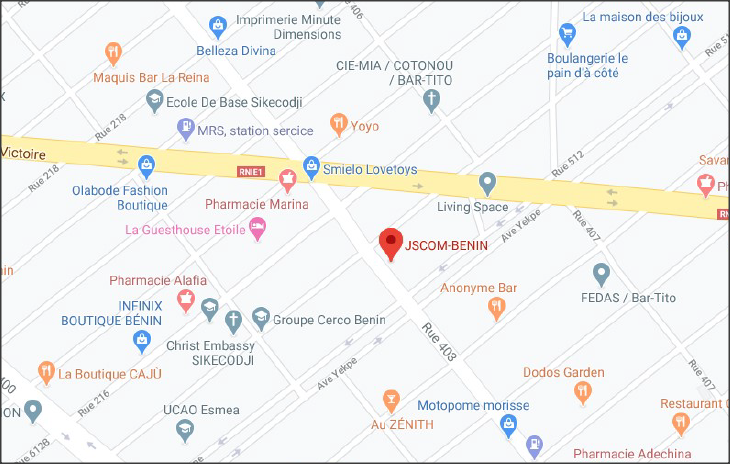
\includegraphics[scale=0.8]{figure/jscom-map.png}		
	\caption{Situation géographique de JScom, source Google maps.}		
	\label{Situation géographique de JScom}
	\end{figure}
		
	 %\subsection{Domaine d'intervention}
		%JScom intervient :
	%\begin{itemize}
		%\item Dans le développement des solutions sur mesure à l'intégration des systèmes d'informations
	%	\item Dans la formation en Windev et Webdev 
	%\end{itemize}
		
	%\section{Déroulement et observations}
\section{Démarche méthodologique}
	Au cours du stage , il a fallu :
	\begin{itemize}
		\item Faire une revue littéraire sur les notions du réseau informatique ;
		\item  Prendre connaissance de la tâche à effectuer ;
		\item Me référer à mes connaissances reçues en classe ;
		\item Effectuer les opérations sur le terrain ;
		\item Faire le traitement au bureau ;
		\item Faire des recherches sur le net  ;
		\item Faire des recherches documentaires ;
		\item Lire beaucoup de cours ;
		\item Surtout Pratiquer.
	\end{itemize}
			
\chapter{Cadre théorique et méthodologique}
	Dans ce chapitre, je vais présenter le thème et toutes les notions fondamentales qui ont rapport au thème.
	
	\section{Contexte et énoncé du problème}
	%J'ai enlevé beaucoup de problème % L'idée aussi est d'amener à combiner le numérique avec l'existent
	J'ai constaté qu'il a beaucoup d'incompréhensions dans la programmation des cours à ENEAM. Les étudiants s'embrouillent sur l'effectivité de la tenue des cours. De même quand on annule un cours les élèves sont parfois mals informés. %Souvent ils sont à l'école et attendent le professeur qui annonce qu'il ne viendra pas. 
	Souvent ils sont à l'école et s'amusent et perdent leur temps à ne rien faire. L'administration diffuse certaines informations qui sont sur support papier et sont collées. Et tout le monde n'est pas au courant; je me rappelle en 3\up{e} année, un de mes camarades est venu très en retard à une composition parce qu'il n'était pas informé de la date des évaluations. Que puis-je faire ? Les étudiants ont besoin d'un moyen de communication puissant pour discuter et ou s'échanger à propos des cours. Comme moyen, il a les réseaux sociaux. Les réseaux sociaux ne répondent pas à ce problème. En effet, on peut communiquer de façon illimitée par les réseaux sociaux, ce qui poussent les étudiants à dirent des inepties par ces canaux. Nous avons donc besoin d'un système qui va remplir plusieurs conditions :
\begin{itemize}
	\item Les professeurs pourront communiquer la programmation des cours aux apprenants de façon efficace ;
	\item Les élèves pourront échanger de façon simple ;
	\item Les administrateurs pourront surveiller le flux d'informations qui transite par le réseau ;
	\item L'administration pourra diffuser des informations et des communiqués ;
	\item L'administration pourra renforcer la qualité de service: on pourrait créer un canal spécial et périodique pour certaines procédures telles que les procédures de réclamation et autres services disponibles temporairement ;
	\item Un système de communication sûre, multi-utilisateurs, sécurisée. 
\end{itemize}

	Etudions les options dont on dispose. En informatique, on pourrait contribuer en réalisant une application, un réseau social.
Présentons ces avantages. Une bonne application peut répondre à tous les problèmes mentionnés ci-dessus mais la conception est une tâche bien pénible surtout lorsqu'on parle de sécurité, de système multi-utilisateurs, multitâches et d'administration. Il suffit pour s'en convaincre d'observer les médias sociaux qui existent : c'est beaucoup % j'ai enlevé d'ingénieurs et 
de technologies réunies. Nous voyons bien que cette solution bien que réalisable, pour qu'elle réponde à tous nos besoins, il faut beaucoup de ressources. Quand on dit ressources ici il y'a les ressources matérielles, humaines , le temps, etc. Au vu de tous ces disconvenues essayons de trouver une autre solution. Comme je suis un étudiant en administration réseaux, je vais essayer de parcourir parmi les solutions que proposent l'incroyable monde du réseau.

	Prenons le mail. Le e-mail ou courrier électronique est un système de transmission de messages électroniques entre différents utilisateurs. Ce système achemine les messages entre deux nœuds reliés entre eux par le réseau internet. Par message électronique, on comprend des messages textes mais aussi des messages enrichis (c'est à dire des messages formatés dans un langage de description des données : HTML \label{ref:html} ), des fichiers joints ( documents , musique , vidéo) et tout autre type de fichiers. Le mail a plusieurs avantages :
\begin{itemize}
	\item C'est un réseau centralisé: les administrateurs peuvent donc surveiller le flux réseau, limiter le nombre de mails envoyés par les étudiants; ce qui empêche les apprenants d'envoyer des messages jugés inutiles ou des blagues sur le réseau. Plusieurs filtres peuvent être définis pour mieux analyser les données qui transitent sur le réseau ;
	\item Les membres de l'administration  peuvent envoyer le programme des cours, des devoirs aux étudiants, donc tout type d'information ;
	\item les élèves peuvent s'échanger entre eux sur les notions reçues ; 
	\item La sécurité est au point : le mail fait intervenir des protocoles réseaux standardisés et sécurisés qui répondent à tous les principes fondamentaux de la cryptographie. C'est un moyen de communication sûr lorsqu'il est bien configuré ;
	\item il a aussi des avantages personnels: l'apprentissage et l'exploration d'un riche et vaste domaine ainsi que la maîtrise de ces champs d'application.
\end{itemize}

	Au vu de ces avantages, je me propose de mettre en place un serveur de messagerie électronique.
Pour cela, je vais procéder étape par étape. Je vais donc mettre en place un serveur simple Linux, monter les disques durs, installer les services de bases DHCP, DNS, Apache,  MySQL, faire de la virtualisation, faire de la modélisation réseau grâce à GNS3, configurer le mail proprement avec les protocoles SMTP et IMAP, penser à la sécurité en définissant une politique de sécurité, en configurant les firewalls , en utilisant de la cryptographie (chiffrement symétrique , asymétrique , certificat, fonction de chiffrement de mot de passe),  mettre en place la supervision pour prévenir, détecter et corriger les problèmes, programmer également un petit site web d'administrations, écrire des scripts Bash.  
	\section{Objectif}
	L'objectif est de mettre en place un serveur mail opérationnel pour l'ENEAM. De façon spécifique, il s'agit de déployer un serveur de messagerie et d'y proposer un accès par la technologie web.
	\section{Hypothèse}
	Les problèmes de communication liée à la programmation des cours sont dus à l'absence d'un moyen de communication innovant, combinant les technologies de l'information au sein de l'ENEAM.
	\section{Etude théorique}
		\subsection{Définition d'un serveur}
		Un serveur est un ordinateur qui fournit un ou plusieurs services aux clients . Les clients et le serveur communiquent grâces à des protocoles réseaux. En réseau, un protocole est un langage qui est bien défini par des règles et qui permet aux ordinateurs (en réalité tout équipement électronique qui possède une carte réseau) de communiquer. Du point de vu logiciel, un serveur peut être vu comme un logiciel qui fournit un service à d'autres logiciels.

\subsubsection{Les caractéristiques d'un serveur}
Un serveur à généralement les caractéristiques suivantes :
\begin{itemize}
\item Un serveur est allumé 24h/24h ;
\item Très souvent, il ne dispose pas d'un écran , ni d'un clavier , ni d'équipements multimédias ;
\item Un serveur Linux n'a généralement pas d'interface graphique ;
\item Un serveur utilise très souvent un système d'exploitation spécialisé.
\end{itemize}

\subsubsection{Quelques services}
Les serveurs assurent différents services. Citons quelques uns:
\begin{itemize}
\item Transfert de fichier: NFS, Samba, bittorrent, FTP ;
\item Communication : Messagerie instantanée, téléphonie par IP ;
\item Authentification: annuire LDAP ;
\item Web.
\end{itemize}

\subsubsection{Spécification d'un OS seveur}
	Un système d'exploitation de serveur (OS Operating System ) n'est qu'un système d'exploitation optimisé pour l'installation de logiciels serveurs. Les OS serveurs ont les caractéristiques suivantes:
\begin{itemize}
	\item Les OS serveurs ne sont pas configurés avec les fonctions de veilles. En effet les serveurs restent allumés tout le temps ;
	\item Les OS serveurs n'ont pas d'interface graphique pour les systèmes Unix et Linux ;
	\item Ils peuvent gérer des ressources physiques énormes par rapport à un ordinateur personnel. Ils peuvent donc gérer par exemple une machine dotée de plus 1 tera (1 To) de mémoires RAM. Il existe des services de support payants pour les entreprises.
\end{itemize} 
	
\subsection{Disque dur RAID LVM}
RAID est un ensemble de techniques qui visent à répartir le stockage de données sur plusieurs disques physiques afin d'anticiper la défaillance des disques et de limiter les risques de pertes données. Son principe est simple : on regroupe plusieurs disques pour constituer un seul disque dur visible par l'utilisateur. Ainsi lorsque l'un des disques se détériore, il suffit de le changer. On distingue plusieurs architectures RAID :
\begin{itemize}
	\item Le RAID 0: dans cette architecture, si on prend deux disques, les deux travaillent en parallèle. Si un disque est détérioré toutes les données sont perdues ;
	\item Le RAID 1 : Pour deux disques durs physiques A et B , les données sont écrites simultanément sur les deux disques. Ainsi si A se gâte on peut continuer à travailler sans perte de données. Il suffit après de changer le disque A détérioré par un nouvel disque C pour ne pas risquer de perdre les données définitivement au cas où le seul disque restant s'endommage ;
	\item Il existe d'autre architectures RAID.
%\item Le raid 10: c'est une combinaison de RAID 0 et RAID 1. Dans cette architecture nous avons deux disques montés
\end{itemize}

\subsection{Serveur web APACHE}
Un serveur web est le service qui permet d'accéder à des pages web. Tout le web repose sur ce service. On aura à accéder à notre serveur de mail par une interface web. Il faudra donc mettre en place un serveur web. Apache ou plus précisément HTTPD est le serveur web le plus populaire. Il est développé et maintenu par la fondation \emph{Apache}. Il sera installé dans la suite. On va aussi utiliser le serveur web Nginx comme reverse proxy\footnote{Un reverse proxy est un proxy qui filtre les requêtes de l'extérieur à destination d'un serveur interne. Il est utile pour la sécurité et les performances car il permet de gérer aussi un système de cache}.

\subsection{Base de donnée}
Les données des utilisateurs doivent êtres stockées dans une base de donnée. Une base de donnée permet de stocker, de structurer, de gérer et d'accéder aux données de façon sûre, rapide et sécurisée. Un SGBD (Système de Gestion de Base de Donnée) est un logiciel qui manipule une base de donnée. Une base de donnée est un fichier ou un ensemble de fichier qui contient des données bien organisées qui peuvent être lues et manipulées par un SGBD à travers un langage informatique(langage de description ou langage de programmation). On distingue deux principaux types de bases de données.
 \begin{itemize}
 \item Les bases de données relationnels : les données sont stockées dans des tables et sont liées entre elle par des relations. On utilise le langage SQL pour interagir avec les données. Comme SGBD de ce type, on distingue MySQL, PostgreSQL, Oracle, et plein d'autres. En SQL, l'instruction: 
 \begin{minted}[frame = single, breaklines, autogobble, bgcolor=bg, label=SQL]{sql}
 SELECT `nom`, `prenom` FROM `utilisateur` WHERE `utilisateur`.`age` >=18 ; --Permet de sélectionner les nom, prénoms de tous les utilisateurs majeurs.
 \end{minted}
 \item Les bases de donnés NoSQL (Not Only SQL) : ceux sont des bases de données qui n'utilisent pas le modèle relationnel. On  peut citer à titre d'exemple Poids, MongoDB, Cassandra, ElasticSearch.
 \end{itemize}
 
\subsection{Modélisation avec GNS3}
Pour mettre en place notre projet il va falloir la modéliser, c'est à dire représenter toute notre architecture réseau de façon visuelle pour avoir un modèle, un plan représentatif de la solution à déployer. GNS3 est un logiciel libre qui permet de modéliser des architectures réseaux, de simuler des architectures réseaux, de visualiser et de tester le résultat grâce à la virtualisation.
\subsection{Programmation}
Un ordinateur ne comprend que le langage binaire , c'est à dire  1 et 0. Pour pouvoir donc donner une instruction à un ordinateur, il va falloir lui parler son langage qu'il comprend (le binaire). Comme le binaire n'est pas un langage accessible aux humains, on a créé les langages de programmation qui sont des instructions écrites dans un langage accessible à l'homme et qui seront ensuite soient lues , soient compilées, soient interprétées par des programmes spécifiques pour permettre à l'ordinateur de comprendre et donc de réaliser une tâche.
\subsubsection{HTML, CSS, PHP, JAVASCRIPT, JQUERY, BASH}
Les langages de programmation  web sont des langages de programmation qui interviennent dans le web. C'est donc un ensemble de technologie qui permettent de créer des pages web dynamiques.
\paragraph{HTML} est un langage de description. C'est un langage dérivé du XML et qui permet d'écrire une page web statique. 
\paragraph{CSS} est un langage de description qui va permettre de rendre le contenu HTML joli( de faire la mise en forme du contenu).
\paragraph{PHP} est un langage coté serveur, il va permettre de manipuler les données reçues par notre interface web (site web).
\paragraph{JAVACRIPT ET JQUERY :} Javascript est le langage qui va nous permettre de rendre responsive le site web coté client. Jquery est un framework du javascript, c'est donc une brique de code déjà implémenté dont on va se servir pour vite développer notre application.
\paragraph{BASH} est un langage de script qui permet d'exécuter des instructions sur un système d'exploitation Linux. Par exemple, on peut écrire un script bash pour dire d'éteindre un ordinateur dans 10 heures de temps. Il est intégré dans tous les systèmes Linux et ne nécessite aucune installation. Il est essentiel car c'est lui qui va nous permettre de créer ou de supprimer les répertoires des utilisateurs, de vérifier l'état d'un service, d'arrêter ou de redémarrer un service.

\subsection{FTP} 
Pour envoyer le site d'administration que nous allons développé sur le serveur, nous n'allons pas utilisé le terminal mais plutôt utilisé le protocole d'envoi de fichier FTP et se servir d'un client FTP graphique (FilleZilla). 
Le protocole FTP permet l'envoi et la réception de fichiers. Il est très utilisé pour le téléchargement de fichiers. La majorité des dépots Linux utilisent le protocole FTP pour le téléchargement des packages (apt le gestionnaire de paquet Debian télécharge les paquets sur des serveurs FTP).
\subsection{Fonctionnement du mail}
La messagerie informatique fait intervenir plusieurs protocoles réseaux. Il a en effet le protocole SMTP qui permet d'envoyer le message et les protocoles IMAP, POP pour accéder aux données (les mails).
\subsubsection{SMTP}
Le serveur SMTP permet d'envoyer un mail. Enonçons son fonctionnement par un exemple. Si Toto veut envoyer un mail à Baké. Toto a pour adresse mail \textbf{toto@toto.com}. Baké à pour adresse \textbf{bake@gmail.com}. Il va se reproduire les étapes suivantes :
\begin{itemize}
	\item Toto va envoyer le mail depuis son poste à son serveur SMTP. 
	\item Le serveur SMTP de Toto va réceptionner le mail et vérifier s'il lui est destiné (il va vérifier si le destinataire du mail est sur ce serveur, c'est à dire si Baké appartient à ce serveur. toto@toto.com a pour domaine toto.com. et bake@gmail.com a pour domaine gmail.com. toto.com est différent de gmail.com donc les deux comptes mail ne sont pas sur le même serveur ). Si oui, il va enregistrer le mail dans le répertoire de réception des mails de Baké. Si non, il va relayer le mail vers le serveur SMTP de Baké. 
	\item Le serveur SMTP de Baké va recevoir le mail de Toto et le stocker dans le répertoire personnel de Toto.	   
\end{itemize}
\begin{figure}[H]
\centering
\includegraphics[scale=1]{figure/"figure envoi SMTP.png"}
\caption{Principe du SMTP}
\label{Principer du SMTP}
\end{figure}

\subsubsection{ IMAP}
	Pour lire mes mails, je dois pouvoir accéder à mon serveur SMTP et lire les messages à distante. Pour cela on utilise le protocole IMAP qui va se connecter au serveur et récupérer les données et l'afficher dans le logiciel qui permet de lire les mails (un exemple Mozilla Thunderbird, Yahoo mail, Zimbra, Rainloop ). 
\begin{figure}[H]
\centering
\includegraphics[scale=1]{figure/"figure_reception_imap.png"} 
\caption{Réception d'un mail en IMAP}
\label{Reception d'un mail en IMAP}
\end{figure}

Le protocole POP permet aussi de récupérer les mails. La différence majeure entre IMAP et POP est que IMAP est une connexion directe, unidirectionnelle  entre le serveur le client mail tandis que POP est une connexion bidirectionnelle.
\begin{itemize}
	\item Cela signifie qu'avec IMAP les données sont sur le serveur et on y accède directement et toute modification faite sur les mails depuis le client mail impacte le serveur (est réalisée sur le serveur). En IMAP, si je supprime des mails depuis mon client mail, les mails sont aussitôt supprimés sur le serveur. De même avec IMAP, il est impossible d'avoir une copie local des mails . On ne peut donc accéder aux mails qu'on a déjà lu sans connexion internet.
	\item Avec POP, on se connecte et on réalise une copie locale de tous les mails qui sont sur le serveur. Ensuite, en interne on peut modifier ses mails sans enregistrer les modifications sur le serveur. On peut lire tous les mails téléchargés hors connexion.  
\end{itemize} 
	Il est conseillé de préférer le protocole IMAP au protocole POP car si on crée plusieurs copies locales d'un mail qui est sur le serveur, on peut facilement se tromper et écraser après des données sur le serveur sans le vouloir. Ou même supposons que j'ai récupéré en POP le mail identifié par \emph{MAIL1} avec mon ordinateur portable. J'ai naturellement commençé par répondre à se mail et j'ai enregistré le brouillon de la réponse \emph{REPONSEMAIL1} sans avoir à envoyer la réponse au serveur. Je sors après sans mon pc et je réalise que je veux envoyer la réponse rédigée précédemment. Je me connecte à mon serveur mail avec mon portable et je ne retrouve par ce brouillon car le brouillon  \emph{REPONSEMAIL1} est enregistré sur mon pc et non sur mon serveur mail. Il m'est donc impossible d'envoyer cette réponse sans passer par mon pc ; ce qui n'allait  pas poser problème en IMAP puisque avec ce dernier le brouillon \emph{REPONSEMAIL1} aurait été enregistré sur le serveur. \\
	Le schéma complet de l'envoi et de la réception d'un mail.
\begin{figure}[H]
\centering
\includegraphics[width=483pt]{figure/"figure_envoi_reception_mail.png"} 
\caption{Résumé de l'envoi et de la réception d'un mail} \label{Résumé de l'envoi et de la reception d'un mai}
\end{figure}

\subsection{Sécurité}
En matière de sécurité on ne peut pas faire confiance aux utilisateurs et donc aux données reçues par les utilisateurs. Il faut alors établir des règles de sécurité strictes pour limiter les risques de mauvaises utilisations et de piratage informatique.
\subsubsection{Firewall}
Le firewall (pare-feu en français) est l'instrument qui va permettre de protéger notre serveur contre l'extérieur. Il va installer une barrière entre notre serveur et l'extérieur. On pourra dire par exemple au serveur d'aller sur internet (communication serveur vers extérieur) ou empêcher les utilisateurs depuis l'extérieur à communiquer avec le serveur\footnote{Il a un troisième cas , on traverse le serveur. Dans ce cas le serveur joue le rôle d'un routeur} (communication extérieur vers serveur). On distingue deux types de firewalls : les firewalls matériels et les firewalls logiciels (ou proxy).
\begin{itemize}
\item Le firewall matériel est une protection pour la couche 3 et 4 du modèle OSI. Il filtre le trafic réseau en lisant les entêtes IP et TCP ;
\item Le proxy est un firewall de niveau 6. Il filtre la couche applicatif. C'est lui qui va par exemple bloquer les étudiants à se connecter aux serveurs à minuit (00 heures). Il sert aussi de cache.
\end{itemize}

\subsection*{Conclusion}
Nous allons installer un serveur Linux ubuntu qui va contenir un certain nombre de services :
\begin{itemize}
	\item  Un serveur SMTP et IMAP pour l'envoi et la réception des mails ;
	\item  Un serveur web pour envoyer les mails depuis une application web (un webmail) ;
	\item  Un site web d'administration pour créer des comptes mails et réaliser quelques tâches d'administration ;
	\item Une base de donnée pour sauvegarder les informations d'authentification ; 
	\item Un serveur FTP pour envoyer les données du site d'administration sur le serveur.
\end{itemize}
Nous allons :
\begin{itemize}
	\item Coder le site web en PHP et en javascript. Les mails seront stockés sur un disque dur RAID\label{ref:raid}, LVM\label{ref:lvm} ;
	\item Ecrire des règles firewalls pour protéger le serveur ;
	\item  Configurer un antispam pour empêcher les spammeurs (Spamassassin) ;
	\item Sécuriser toute la communication par le chiffrage et des certificats ;
	\item Utiliser comme nom de domaine eneam.da\footnote{On pourra changer après ce nom en production}. Le webmail aura pour adresse www.eneam.da et le site d'administration www.admin.eneam.da.
\end{itemize}

%CHAPITRE CONCERNANT L'IMPLEMENTATION
\chapter{Implémentation du projet}
Je vais dans un premier temps me mettre dans la peau d'un administrateur système et configurer tous les services réseaux. Dans un second temps, dans la section \ref{ref:casConret} à la page \pageref{ref:casConret}, je vais me mettre à la place de l'utilisateur du système et je vais créer des comptes mails et envoyer des mails de façon simple et pratique. 
\section{Installation du serveur}
Nous allons utilisé pour notre travail comme OS \href{https://ubuntu-fr.org/telechargement?variante=server}{Ubuntu Server} et VMware comme hyperviseur\footnote{Un hyperviseur est un logiciel qui fournit un environnement virtuel pour installer un OS sans avoir un matériel réel. C'est grâce au hyperviseur qu'on pourra installer Linux et tester notre projet depuis un poste Windows}. Ubuntu est une distribution Linux gratuite et très populaire. Nous allons utiliser la version  LTS d'Ubuntu Server qui est disponible sur le site d'Ubuntu . La version LTS signifie Long Term Support qui correspond à une version d' Ubuntu qui sort tous les 2 ans et qui bénifie d'un support étendu sur 5 ans. L'avantage est qu'on ne va pas s'embêter avec des mises régulières comme avec un OS standard. Le choix de l'hyperviseur VMware est axé sur le fait qu'il supporte une meilleure intégration avec l' émulateur d'architectures réseaux GNS3.%\footnote{sera détaillé dans la suite}. 

%\subsection{Installation du serveur}
	On installe d'abord l'hyperviseur VMware workstation. Pour cela rien de plus simple on se rend sur le site de VMware en cliquant \href{https://my.vmware.com/en/web/vmware/free}{ici}. On télécharge et installe le logiciel. On ouvre le logiciel. J'utilise la version en anglais de VMware. On ouvre l'onglet File ensuite "New virtual Machine". Une fenêtre s'ouvre et nous suivons le guide durant la configuration de la nouvelle machine virtuelle. Les étapes d'ajout d'une machine virtuelle sont disponibles sur le site de VMware. Nous avons normé la machine virtuelle serveur et elle à les configurations suivantes 1 Go de mémoire RAM , 40Go de stockage de masse (disque dur).

	On démarre la machine virtuelle \emph{\textbf{"serveur"}} avec le disque virtuel Ubuntu Server qu'on a téléchargé \href{https://my.vmware.com/en/web/vmware/free}{ici} pour démarrer l'installation. On suit les instructions (on choisit la langue, le clavier, on configure le réseau en DHCP). A la fin de l'installation le système nous dit de redémarrer. Après redémarrage, on entre le nom d'utilisateur et le mot de passe. Il faut configurer le réseau. 
Pour cela il faut déjà avoir d'interfaces réseaux dans la machine virtuelle. On éteint la machine avec la commande 
\begin{exempleConsole}
	sudo shutdown now 
\end{exempleConsole}
Dans VMWare on édite les paramètres de la machine virtuelle et on lui ajoute % deux adaptateurs réseaux en veillant à bien cocher la case Custom et choisir VMnet2 pour le premier adaptateur et pour le second on choisit NAT.
un adaptateur réseau (on choisit NAT). La NAT va permettre à notre machine d'avoir accès à internet\footnote{cela sera modifié au moment des configurations avec GNS3}. On démarre la machine. On tape la commande
\begin{exempleConsole}
netplan apply
\end{exempleConsole}

\section{Gestion du stockage de fichier}
	Nous allons configurer un disque dur spécial pour les données liées aux mails que le serveur va contenir.
	
\subsection{Système de fichier}
	Toutes les données contenues dans un ordinateur sont du binaires( suite de 0 et 1). Il n'a aucun moyen pour un homme de distinguer alors les données. Pour cela on a créé les fichiers. Un fichier est alors un contenu (ou un conteneur de données) binaire qui porte un nom et a une extension qui permet de le distinguer. Ainsi, il est facile pour un homme de reconnaître une image par son extension jpeg ou un document word par docx. Les fichiers sont stockées sur un stockage de masse (disque dur, carte mémoire). Un système de fichier est un index qui définit comment les fichiers sont stockés et organisés sur le stockage afin de permettre et faciliter l'accès aux différents fichiers. On distingue différents systèmes de fichiers fat32 ,NTFS ext3, ext4. EXT4 est l'actuel système de fichier qui est utilisé sur Linux. Il n'est pas compatible Windows, c'est à dire que Windows ne supporte pas le système de fichier EXT4. Donc pour pouvoir stockés des informations sur un disque dur, il faut d'abord le préparer. Cela se fait créant le système de fichier puis en formatant le disque dur.
\subsection{Ajout de disque dur au serveur}	
	On éteint le serveur. Puis on va dans les paramètres de la machine virtuelle ensuite on ajoute trois disques de 2 giga configurés en SCSI\footnote{ est une spécification matérielle des disques}.\\
On redémarre la machine ensuite on exécute les instructions suivantes : \\
On affiche la liste des disques durs. 
\begin{exempleConsole}
ls -la /dev/sd* 
\end{exempleConsole}

Ensuite on verifie la taille de chaque disque avec la commande
\begin{exempleConsole}
gdisk dev/sdb
\end{exempleConsole}

 Dans gdisk on fait p pour afficher la structure du disque pour être sur que c'est deux giga. q  pour quitter. On reprend avec les deux autres disques dur montés. \\
 On crée le raid 1 avec la commande  
\begin{exempleConsole}
mdadm --create /dev/md0 --level=raid1 --raid-devices=2 /dev/sdb /dev/sdc spare-devices=1 /dev/sdd
\end{exempleConsole}

On affiche les détails sur le nouveau disque raid créé et on copie l'identifiant UUID
\begin{exempleConsole}
mdadm --query --detail /dev/md0
/dev/md0:
           Version : 1.2
     Creation Time : Wed Dec 25 14:33:47 2019
        Raid Level : raid1
        Array Size : 2094080 (2045.00 MiB 2144.34 MB)
     Used Dev Size : 2094080 (2045.00 MiB 2144.34 MB)
      Raid Devices : 2
     Total Devices : 3
       Persistence : Superblock is persistent

       Update Time : Tue Mar 10 11:18:38 2020
             State : clean
    Active Devices : 2
   Working Devices : 3
    Failed Devices : 0
     Spare Devices : 1

Consistency Policy : resync

              Name : serveur:0  (local to host serveur)
              UUID : 1bf998cb:0b420815:25812e34:403d63c5
            Events : 26

    Number   Major   Minor   RaidDevice State
       0       8       16        0      active sync   /dev/sdb
       1       8       32        1      active sync   /dev/sdc

       2       8       48        -      spare   /dev/sdd

\end{exempleConsole}

On ajoute la ligne suivante dans le fichier /etc/mdadm/mdadm.conf pour que le disque dur ne change pas de nom lors du prochain démarrage
\begin{exempleConsole}
ARRAY /dev/md0 level=raid1 num-devices=2 spares=1 UUID=1bf998cb:0b420815:25812e34:403d63c5 devices=/dev/sdb,/dev/sdc,/dev/sdd
\end{exempleConsole}

Pour que les modifications soient effectives au prochain démarrage du système on fait 
\begin{exempleConsole}
sudo update-initramfs -u
\end{exempleConsole}

On passe au partitionnement du nouveau disque avec LVM
\begin{exempleConsole}
sudo pvcreate /dev/md0
sudo vgcreate raid-volume /dev/md0 
sudo lvcreate --name data --size 2000M raid-volume
\end{exempleConsole}
Il faut maintenant monter la partition. Pour cela on crée le dossier de montage de la partition puis on monte notre partition \emph{\textbf{data}} dans ce dossier 
\begin{exempleConsole}
mkdir -p /externe
mount -t ext4 /dev/raid-volume/data /externe
\end{exempleConsole}

Il faut rendre automatique le montage de la partition permenent à chaque démarrage du système. On édite le fichier /etc/fstab et on ajoute la ligne
\begin{exempleConsole}
/dev/raid-volume/data /externe ext4 defaults 0 0
\end{exempleConsole}

\section{Configurer le LAMP}
On va installer PHP, MariaDB qui est un fork\footnote{C'est quand des développeurs d'un logiciel en général libre n'étant plus d'accord pour continuer le projet se séparent et créent leur propre version du logiciel à partir du code source de départ.} de MySQL.
\begin{exempleConsole}
sudo su
apt-get update #Pour mettre à jour le cache local
apt-get install apache2 libapache2-mod-php php-fpm mysql-server libapache2-mod-rpaf
#Pour activer les modules apache nécessaires
sudo a2enmod proxy_fcgi setenvif
sudo a2enconf php7.2-fpm
sudo a2dismod php7.2 mpm_prefork
sudo a2enmod mpm_event
sudo systemctl restart apache2
\end{exempleConsole}
\subsection{Gestion de Apache}
Nous changeons les ports sur lesquels écoute Apache httpd et il écoutera sur 7080 pour le http et 7443 pour le https en local. L'avantage est que notre serveur apache n'est pas exposé à l'extérieur. On verra seulement notre reverse-proxy Nginx de l'extérieur. On modifie le fichier /etc/apache2/ports.conf
\exempleConsoleFileBash{source/apache-ports.conf}
Nous allons configurer les virtualhosts (c'est à dire les deux sites web qui seront hébergés sur le serveur). Ces sites seront sécurisés avec des certificats autosignés\footnote{Un certificat autosigné est un certificat qui n'est pas créé par une autorité de certification.}.\label{ref:rainloop}
Pour le client webmail qui va permettre l'envoi des mails, on crée le fichier /etc/apache2/site-available/www.eneam.da.conf
\exempleConsoleFile{source/www.eneam.da.conf}
Pour le site d'administration /etc/apache2/site-available/www.admin.eneam.da.conf
\exempleConsoleFile{source/www.admin.eneam.da.conf}
On crée aussi les dossiers /externe/www/html/www.admin.eneam.da/logs/ récursivement.
\begin{exempleConsole}
mkdir -P /externe/www/html/www.admin.eneam.da/logs/ /externe/www/html/www.admin.eneam.da/public_html/
\end{exempleConsole}
Nous n'avons pas activé ces virtualhosts pour le moment sinon Apache va sortir une erreur.
\subsection{Gestion de Nginx}
\begin{exempleConsole}
sudo apt-get install nginx libapache2-mod-rpaf
\end{exempleConsole}
Il faut créer les  \textbf{“server blocs”}\footnote{Dans Nginx on appelle les virtualhosts server blocs.} associés à nos virtualhosts. Pour le premier /etc/nginx/site-available/www.admin.eneam.da
\exempleConsoleFileBash{source/www.admin.eneam.da}
Le fichier /etc/nginx/site-available/www.eneam.da
\exempleConsoleFileBash{source/www.eneam.da}
\subsection*{Résumé}
En somme, nous avons configuré un serveur web Nginx accessible depuis l'extérieur. Lorsqu'on va se connecter aux différents sites depuis un navigateur, les requêtes(HTTP et HTTPS pour être précis) sont envoyés à Nginx. Nginx filtre  ces requêtes et va ensuite rediriger les requêtes en interne vers Apache. Apache en traitant ses requêtes, va déléguer le traitement des scripts PHP au processus FastCGI \emph{\textbf{PHP-FPM}}. Tout ceci se fait de façon transparente pour l'utilisateur.
\begin{figure}[H]
	\centering
	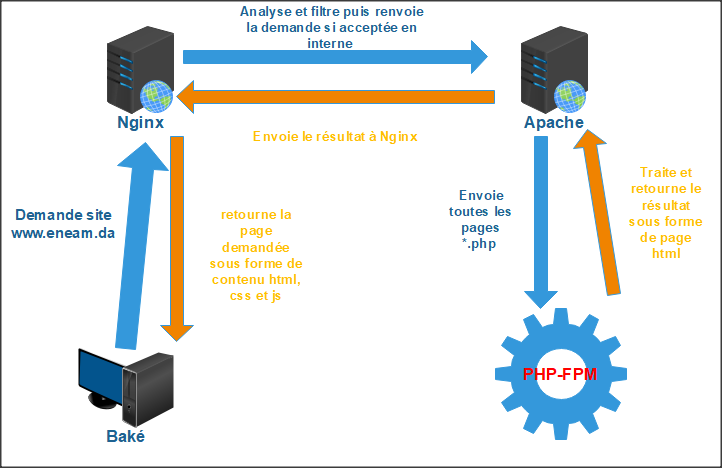
\includegraphics[scale=0.7]{figure/resume-fonctionnement-web-eneam.png}
	\caption{Résumé du fonctionnement web du réseau projetmail}	
\end{figure}

\section{Modélisation de l'architecture réseau avec GNS3}
	On télécharge les logiciels GNS3  et  GNS3 VM sur le site officiel de GNS3. On istalle GNS3.
On lance le logiciel VMWare et dans VMWare on fait :
\begin{itemize}
	\item Fichier puis ouvrir fichier ;
	\item  On choisit le fichier GNS VM au format ova téléchargé ;
\end{itemize}
Cela va installer une nouvelle machine virtuelle. Il faut ensuite importer cette machine dans le logiciel GNS3.
\begin{itemize}
	\item On lance GNS3. Menu Edit -> Préférences -> GNS3 VM ;
	\item On coche la case  “Enable the GNS3 VM” et on sélectionne “VMware Worstation/Player” dans le champ Virtualize engine ;
	\item Cliquez sur Refresh et GNS3 VM apparaît dans VM name ;
	\item Cliquez sur Apply.
\end{itemize}
On va ajouter notre machine Linux \emph{\textbf{"serveur"}} de VMware pour l'utiliser lors de la modélisation
\begin{itemize}
	\item Dans Preferences -> VMware -> VMware VMs -> new ;
	\item Une fenêtre apparaît on coche run this VMware VM on my local computer puis next ;
	\item Dans VM list on choisit la machine serveur un clic sur le bouton finish.
\end{itemize}

\subsection{Description du schéma}
\begin{figure}[H]
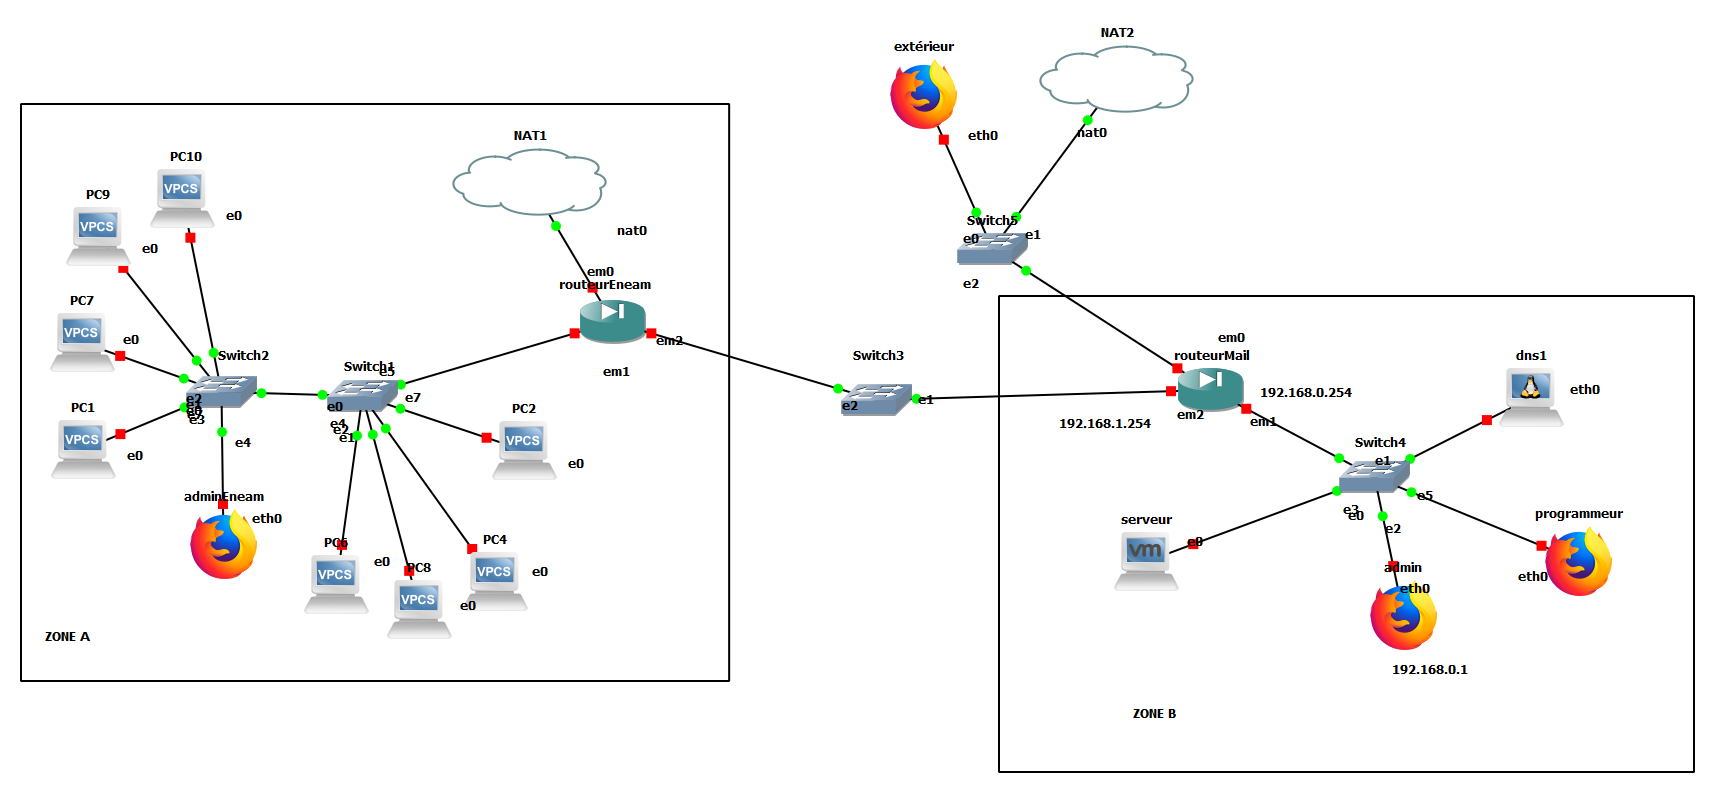
\includegraphics[width=520pt]{figure/topologie_gns3.png}
\centering
\caption{Topologie de notre projet dans GNS3}	
\end{figure}	
Nous avons opté pour un modèle générique. Le réseau est séparé en deux grandes parties: la zone A et la zone B
\begin{itemize}
\item La zone A : représente le réseau existant de l'ENEAM. Il est géré par \emph{\textbf{routeurEneam}} et est relié au routeur routeurMail. La configuration de cette zone ne nous intéresse pas. Elle permet de mieux comprendre l'architecture de notre projet et de comprendre que notre projet est générique car il peut s'adapter à tout type d'organisation existante sans toucher au système d'information\footnote{ Un système d'information est un ensemble de ressources matérielles, humaines qui permet de collecter, de stocker, de traiter et de diffuser l'information.} existant.
\item La zone B: le nouveau réseau relié par le routeur routeurMail.
L'avantage d'une telle architecture est que l'administrateur du réseau ENEAM peut communiquer avec le réseau mail à travers un tunnel (VPN) s'il est configuré.
\item \textbf{routeurEneam} procède trois interfaces réseaux : em1 dans son réseau local, em2 qui le relie à routeurMail et em0 pour le WAN ;
\item \textbf{routeurMail} de même à trois interfaces ;
\item \textbf{dns1} est un docker\footnote{Est un conteneur qui contient un service et toutes les dépendances de ce dernier. Il permet d'isoler le service qu'on veut déployer(ici DNS) sans avoir à s'encombrer d'autres services dont on a pas besoin. Sans un docker, on aurait à installer un autre serveur Linux juste pour le DNS mais qui contient déjà plein de programmes dont nous n'avons  pas besoin. En somme un docker contient le strict minimum} qui contient un petit serveur DNS qui va servir à la résolution dynamique des noms de domaine au sein du réseau local ;
\item \textbf{serveur :} c'est notre serveur ubuntu installé depuis VMware ;
\item \textbf{routeurMail} et \textbf{routeurEneam} sont des routeurs Pfsense\footnote{Est un routeur firewall open source.} ;
\item \textbf{NAT2} permet de connecter routeurMail à internet et de pouvoir simuler l'accès de notre architecture à internet. Notre routeur aura un adressage privé (pour em0) ce qui n'est pas le cas dans la réalité puisque em0 devait avoir une adresse publique directement accessible sur internet. En effet, la modélisation avec GNS3 nous impose de faire comme cela ;
\end{itemize}

Les étapes de la créations du projet :
\begin{itemize}
\item On crée un nouveau projet "projetmail" ;
\item On ajoute tous les équipements à notre topologie ;
\item On démarre et configure routeurEneam ;
\item on configure le serveur DNS sur le poste \textbf{dns1} ;
\item On accède à routeurEneam depuis le poste admin et on configure la NAT et le port forwading ( redirection de port en français). Pour cela:
	\begin{itemize}
	\item Depuis le poste \textbf{admin},on ouvre le navigateur Firefox ;
	\item On tape l'adresse 192.168.0.254 et on accède à routeurEneam. Les identifiants par défaut sont admin et pour mot de passe pfsense. On change le mot de passe par défaut.
	\begin{figure}[H]
	\centering
	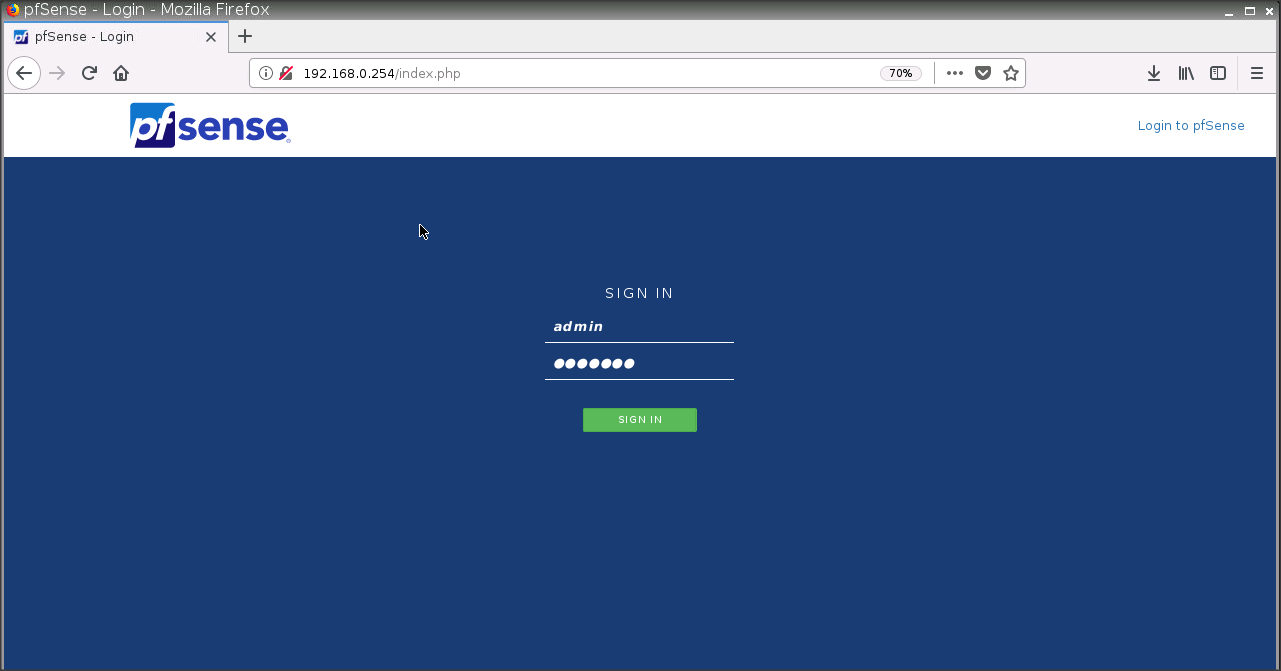
\includegraphics[width=483pt]{figure/pfsense_login.png}
	\caption{Connexion à pfsense par un navigateur}	
	\end{figure}	 	
	\end{itemize}
Ce qu'on a fait va permettre d'accéder au mail par le webmail mais aussi d'accéder par d'autre clients mail tels que Mozilla Thunderbird puisqu'on a rendu directement les ports STMP et IMAP ouverts vers l'extérieur. Si on fermait ces ports, il serait impossible de s'envoyer des mails sans passer par un client webmail installé sur le serveur
\begin{figure}[H]
\centering
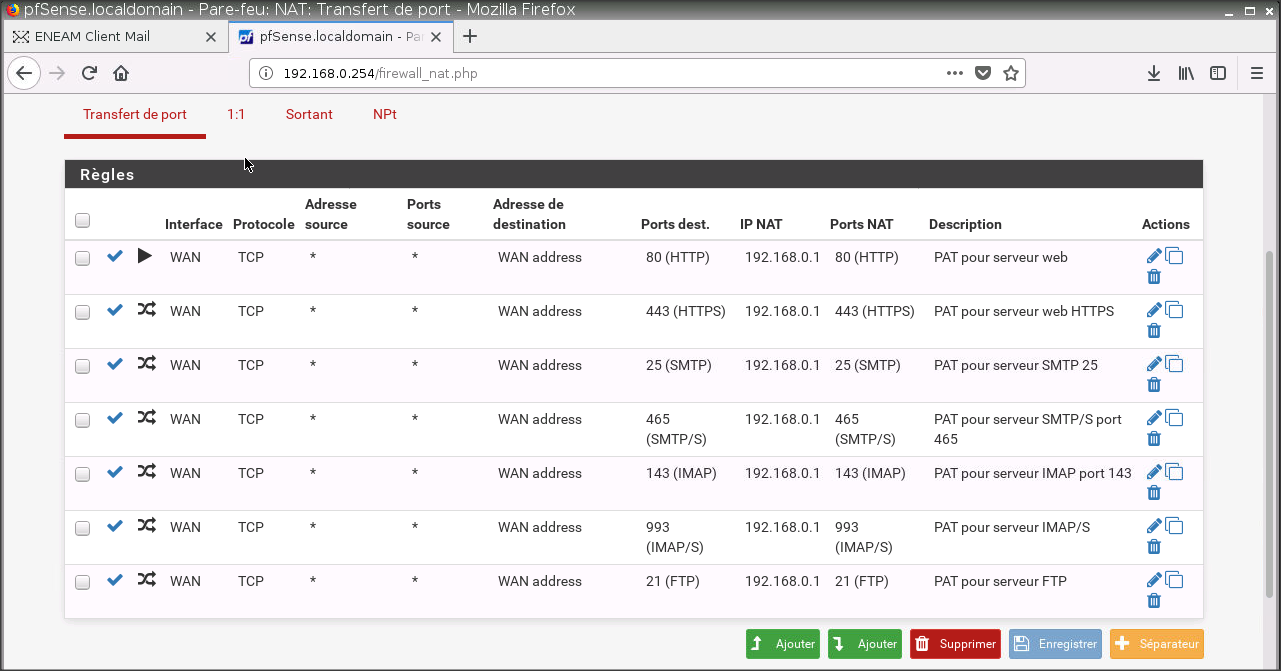
\includegraphics[width=483pt]{figure/figure_routeurMail_configuration_pat.png}
\caption{Configuration du port forwarding}
\label{Configuration du PAT}
\end{figure}
\item Il faut modifier les interfaces réseaux de notre serveur nommé \emph{\textbf{serveur}}. Pour cela dans VMware, on le configure pour qu'il ait deux interfaces réseaux ; l'une représente son interface dans lequel il est connecté dans GNS3 (e0 selon notre schéma) et la seconde interface est configuré en Host-Only\footnote{En effet, le site d'administration est codé sur ma machine physique Windows, il faut un moyen pour pouvoir envoyer le site sur le serveur virtuel, alors on a créé un réseau privé entre le serveur de VMware et mon ordinateur Windows}. On crée aussi le fichier /etc/netplan/60-lan\_statique.yaml pour configurer les interfaces du serveur.
\exempleConsoleFileYAML{"source/60-lan_statique.yaml"}
\end{itemize}

% peut servir à supprimer plus tard
%Postfix est un serveur SMTP. C'est donc lui qui va servir à l'envoi des mails
%Prenons le poste PC1 du réseau em1 s'il veut envoyer un mail à  jean@eneam.da
%depuis son poste il passe par internet. Il n'a pas communication directe entre les deux routeurs pour des  utilisateurs locaux.
%Il se connecte au serveur mail
\subsection{Configuration des équipements}

\section{Installation Postfix}
L'installation du serveur SMTP Postfix va se faire toujours avec notre gestionnaire de paquet apt
\begin{exempleConsole}
apt-get install postfix  postfix-mysql #et on reponds aux boites de dialogues qui s'affiche
\end{exempleConsole}

Les fichiers de configuration de postfix sont dans le dossier /etc/postfix/.
On fait une copie des fichiers de configuration avant toute modification.
On modifie le fichier /etc/postfix/main.cf
\exempleConsoleFile{source/postfix-main.cf}
Dans ce fichier :
\begin{itemize}
	\item le serveur postfix écoute sur IPV4 et IPV6 ;
	\item la partie SASL AUTHENTIFICATION renforce la sécurité du serveur. En effet SASL est un protocole qui permet de sécuriser une connexion non sécurisée ;
	\item la partie TLS renforce la sécurité du serveur. SSL est un protocole qui va aussi permettre de sécuriser le serveur ;
	\item Toujours pour la sécurité on utilise des certificats autosignés ; 
	\item la propriété virtual\_mailbox\_domains = mysql:/etc/postfix/sql/mysql-virtual-mailbox-domains.cf définie le fichier qui va contenir la directive de connexion à notre base de donnée mysql plus précisément MariaDB ;
	%\item virtual\_mailbox\_maps = mysql:/etc/postfix/sql/mysql-virtual-mailbox-maps.cf.	
	\item la partie utilisation de boite virtuelle va permettre d'utiliser les virtualhosts c'est à dire des comptes mails virtuels qui ne représentent pas les mails des utilisateurs réels de la machine \textbf{serveur}. L'utilisateur vhosts est créé par la commande
	\begin{exempleConsole}
	groupadd -g 5000 vhosts 
	useradd -g vhosts -u 5000 vhosts -d /externe/mail/vhosts -s /bin/false -m
	\end{exempleConsole}
\end{itemize}

Le fichier mysql-virtual-mailbox-domains.cf contient 
\begin{exempleConsole}
user = messagerieUser
password = isidore
hosts = 127.0.0.1
dbname = messagerie
query = SELECT 1 FROM virtual_domains WHERE name='%s'
\end{exempleConsole}
Le fichier mysql-mailbox-map contient 
\begin{exempleConsole}
user = messagerieUser
password = xxxxxxx
hosts = 127.0.0.1
dbname = messagerie
query = SELECT maildir FROM virtual_users WHERE email='%s'
\end{exempleConsole}
Le cerficat est créé grâce à la célèbre bibliothèque  cryptographique openssl.
\begin{exempleConsole}
openssl req -x509 -nodes -days 365 -newkey rsa:2048 -keyout /etc/ssl/private/dovecot-autosigne.key -out /etc/ssl/certs/dovecot-autosigne.crt
\end{exempleConsole}
Nous modifions le fichier master.cf. Il va permettre toujours de renforcer la sécurité et d'obliger le serveur à accepter que des connexions sécurisées
\exempleConsoleFile{source/postfix-master.cf}
Les directives spamassassin permettent d'indiquer à Postfix d'utiliser spamassassin comme filtre antispam.
%\subsection{Création de la base de donnée des tables}
\section{Installation de Dovecot}
Dovecot est un serveur IMAP et POP 
\begin{exempleConsole}
apt-get install dovecot-core dovecot-imapd dovecot-mysql dovecot-lmtpd dovecot-pop3d
\end{exempleConsole}
Dans allons dans le dossier de configuration de dovecot /etc/dovecot/ .
Nous modifions le fichier /etc/dovecot/conf.d/10-mail.conf dans lequel nous allons éditer deux lignes :
\begin{exempleConsole}
mail_location = maildir:/externe/mail/vhosts/%d/%n
mail_uid = vhosts
mail_gid = vhosts
mail_privileged_group = mail
first_valid_uid = 5000
last_valid_uid = 5000
\end{exempleConsole}
On modifie le fichier /etc/dovecot/conf.d/10-auth.conf et on ajoute 
\begin{exempleConsole}
disable_plaintext_auth = yes
auth_mechanisms = plain login
!include auth-sql.conf.ext
\end{exempleConsole}

Le fichier /etc/dovecot/conf.d/auth-sql.conf.ext :
\begin{exempleConsole}
passdb {
  driver = sql
  args = /etc/dovecot/dovecot-sql.conf.ext
}
userdb {
  driver = static
  args = uid=vhosts gid=vhosts home=/externe/mail/vhosts/%d/%n
}
\end{exempleConsole}

Le fichier /etc/dovecot/dovecot-sql.conf.ext :
\begin{exempleConsole}
driver = mysql 
default_pass_scheme = ARGON2I
connect = host=127.0.0.1 dbname=messagerie user=messagerieUser password=AMETTRE
password_query = SELECT email as user, password FROM virtual_users WHERE email='%u'
\end{exempleConsole}
Le fichier 10-master.conf
\begin{exempleConsole}
service imap-login {
  inet_listener imap {
    #port = 143
  }
  inet_listener imaps {
    #port = 993
    #ssl = yes
  }
}
service pop3-login {
  inet_listener pop3 {
    #port = 110
  }
  inet_listener pop3s {
    #port = 995
    #ssl = yes
  }
}
service submission-login {
  inet_listener submission {
    #port = 587
  }
}
service lmtp {
    unix_listener /var/spool/postfix/private/dovecot-lmtp {
    mode = 0600
    user = postfix
    group = postfix
  }
}

service imap {
}
service pop3 {  
}
service submission {
  # Max. number of SMTP Submission processes (connections)
  #process_limit = 1024
}
service auth {
  unix_listener auth-userdb {
    mode = 0600
    user = vhosts
    group = vhosts 
  }
  # Postfix smtp-auth
  unix_listen  er /var/spool/postfix/private/auth {
    mode = 0666
    user = postfix
    group = postfix 
}
}
service auth-worker {
  
}
service dict {
  unix_listener dict {
    mode = 0600
    user = vhosts
    group = vhosts
  }
}
\end{exempleConsole
Le fichier /etc/dovecot/10-ssl.conf va contenir les informations pour sécuriser le serveur avec les certificats :
\begin{exempleconsole}
ssl = yes
ssl_cert = </etc/ssl/certs/dovecot-autosigne.pem
ssl_key = </etc/ssl/private/dovecot-private-autosigne.pem
ssl_dh = </etc/ssl/certs/dovecot-dh-autosigne.pem
ssl_prefer_server_ciphers = yes
\end{exempleConsole}
\section{Installation du client mail}
\begin{exempleConsole}
mkdir -p /externe/www/rainloop/public_html /externe/www/rainloop/logs 
cd /var/www/rainloop/public_html 
curl -sL https://repository.rainloop.net/installer.php | php
\end{exempleConsole}
Le virtualhost associé à rainloop dans Apache a déjà été créé dans la section \ref{ref:rainloop} à la page \pageref{ref:rainloop}. 
Il faut activer ce virtualhost
\begin{exempleConsole}
ln -s /etc/nginx/sites-available/www.eneam.da.conf /etc/nginx/sites-enabled/www.eneam.da.conf
#On active tous les autres virtualhosts
ln -s /etc/nginx/sites-available/www.admin.eneam.da.conf /etc/nginx/sites-enabled/www.admin.eneam.da.conf
a2ensite www.eneam.da.conf www.eneam.da.conf
systemctl restart nginx apache2 php7.2-fpm 
\end{exempleConsole}
On change le propriétaire et les droits d'accès aux répertoires pour permettre aux utilisateurs d'accéder aux sites.
\begin{exempleConsole}
chown -R www-data:www-data /erterne/www/html/www.admin.eneam.da/ 
chown -R www-data:www-data /erterne/www/rainloop/public_html/
chmod -R 660  /erterne/www/html/www.admin.eneam.da/  
chmod -R 660 /erterne/www/rainloop/public_html/
\end{exempleConsole}
Nous allons profité pour configurer notre domaine dans rainloop , pour cela:
\begin{itemize}
	\item on tape www.eneam.da/?admin dans le navigateur Firefox depuis le poste admin ;
	\item On entre les identifiants par défaut admin et mot de passe 12345 ;
	\item On change les identifiants ;
	\item On configure la langue en français ;
	\item On ajoute les serveurs SMTP et IMAP de notre domaine en cliquant sur le menu domaine.
\end{itemize} 
\begin{figure}[H]
	\centering
	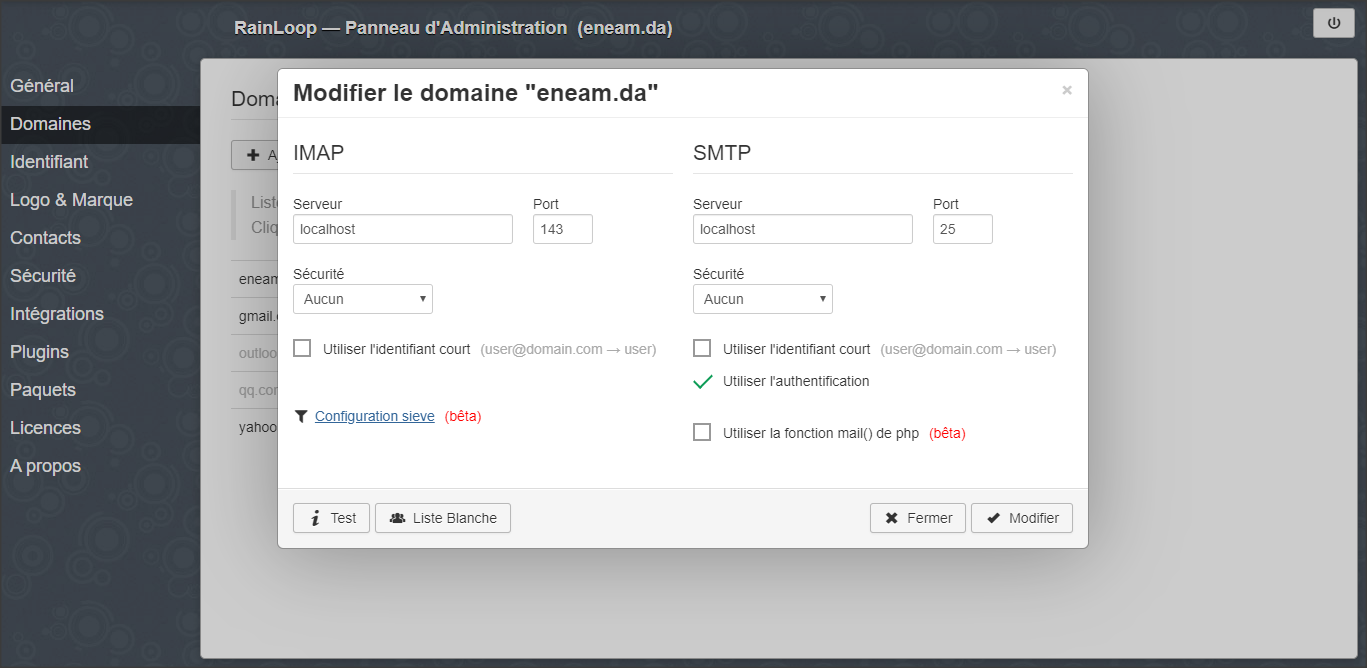
\includegraphics[width=483pt]{figure/configuration-domaine-rainloop.png}
	\caption{Ajout des serveurs mails dans rainloop}
\end{figure}

\section{Le site d'administration}
Le site d'administration va permettre de créer et de supprimer  les comptes emails, de voir la liste de quelques services (SMTP, IMAP , APACHE NGINX ), leur états,  de les arrêter ou de les éteindre. %Il a aussi la fonctionnalité qui va permettre à l'administrateur de voir les mails des étudiants qui est en cours de développement.
Il existe des solutions gratuites pour l'administration du mail comme \emph{\textbf{postfixadmin}}
\subsection*{Pourquoi n'ai-je pas utilisé une solution existante ?}
\begin{itemize}
\item Les solutions existantes contiennent beaucoup de fonctions et parfois d'autres que j'ai jugé inutile dans notre contexte. Prenons les alias. On conçoit difficilement qu'il puisse avoir d'alias de comptes (c'est à dire un alias d'un email ou un étudiant possédant plusieurs comptes).
\item Le bonheur de coder: on va comprendre les principes de base pour coder un site d'administration de mails et écrire des scripts bash; ce qui est très intéressant et montre qu'on arrive à combiner toutes les technologies qu'on nous à enseigner lors des cours et dont on dispose pour produire un résultat ;
\item Postfixadmin est un outils puissant mais son interface est un peu vieillissant ;
\item  La flexibilité: étant donné que nous codons nous allons adapter l'application à notre besoin ;
\item Il existe des outils puissant, complet mais pas gratuit et qui contiennent des fonctionnalités dont on a pas besoin.\footnote{Dans le monde professionnel, on préfèrera des solutions complètes, faciles d'utilisation comme cPanel. Mais ces solutions sont à des prix très onéreux.}
\end{itemize}

L'administrateur du système va exécuter des instructions depuis l'interface web et pour communiquer avec la machine \textbf{serveur} via l'interface web, il va appeler des scripts bash. Nous avons un script bash pour créer le répertoire d'un utilisateur, un autre pour supprimer un répertoire lors de la suppression d'un compte, un autre pour connaître l'état d'un service, un pour arrêter ou redémarrer un service. Voici le contenu du script qui redémarre un service 
\exempleConsoleFileBash{source/restartOrStopService.sh}

Pour permettre l'exécution de script bash depuis le web, il faut autoriser l'utilisateur web \emph{\textbf{www-data}} à lancer des scripts en ayant les droits administrateurs. Pour cela on installe le programme sudo et on ajoute quelques lignes dans le fichier /etc/sudoers
\begin{exempleConsole}
sudo apt-get install sudo 
#Les lignes dans /etc/sudoers
www-data ALL = NOPASSWD: /externe/www/html/www.admin.eneam.da/public_html/scripts/*
# On admet que tous nos scripts qui ont besoins des droits root sont dans ce répertoire	
\end{exempleConsole}

\section{Configuration du FTP  avec vsftpd}
\begin{exempleConsole}
sudo apt-get update
sudo apt-get install vsftpd
\end{exempleConsole}
Le fichier de configuration de vsftpd /etc/vsftpd.conf
\exempleConsoleFile{source/vsftpd.conf}
On crée le dossier /etc/vsftpd/ puis le fichier /etc/vsftpd/programmeur qui va contenir les directives pour connecter l'utilisateur virtuel programmeur au serveur FTP :
\exempleConsoleFile{source/programmeur}
\section{Spamassassin}
Spamassassin est un antispam. Il va lire dans les logs et vérifier le nombre de tentatives de connexion échoué ou autres paramètres. Si ça atteind ou dépasse un seuil, il bloque les connexions du client au serveur. Ce qui empêche les spammeurs d'utiliser le serveur pour envoyer du spam\footnote{Contenu, mail indésirable.}. Plus les règles sont strictes, plus il va rejeter de mails. 
\begin{exempleConsole}
apt-get install spamassassin
\end{exempleConsole}
On crée un utilisateur propre à spamassassin
\begin{exempleConsole}
sudo adduser spamd --disabled-login
\end{exempleConsole}
Le fichier /etc/default/spamassassin sera modifié
\begin{exempleConsole}
ENABLED =1
OPTIONS="--create-prefs --max-children 5 --username spamd --helper-home-dir /home/spamd/ -s /home/spamd/spamd.log"
CRON =1
\end{exempleConsole}
Nous ajoutons les règles dans le fichier /etc/spamassassin/local.cf
\begin{exempleConsole}
rewrite_header Subject [***** SPAM _SCORE_ *****]
required_score 5.0
use_bayes 1
bayes_auto_learn 1
\end{exempleConsole}

\section{La base de donnée MariaDB}
Voici le script sql complet qui gère notre domaine
\exempleConsoleFileSQL{source/script-database-creation.sql}
\section{ Sécurité}
Nous allons écrire des règles iptables 
\begin{exempleConsole}
iptables --policy FORWARD DROP
iptables --policy INPUT  DROP
iptables --policy OUTPUT  DROP
#FTP
iptables --append INPUT --protocol tcp --dport 21 -m conntrack --ctstate NEW,ESTABLISHED -j ACCEPT
#SSH
iptables --append INPUT --protocol tcp --dport 22 -m conntrack --ctstate NEW,ESTABLISHED -j ACCEPT
#SMTP et SMTPS SMTP sur STARTLS
iptables --append INPUT --protocol tcp --dport 25 -m conntrack --ctstate NEW,ESTABLISHED -j ACCEPT
iptables --append INPUT --protocol tcp --dport 465 -m conntrack --ctstate NEW,ESTABLISHED -j ACCEPT
iptables --append INPUT --protocol tcp --dport 587 -m conntrack --ctstate NEW,ESTABLISHED -j ACCEPT
#HTTP et HTTPS
iptables --append INPUT --protocol tcp --dport 80 -m conntrack --ctstate NEW,ESTABLISHED -j ACCEPT
iptables --append INPUT --protocol tcp --dport 443 -m conntrack --ctstate NEW,ESTABLISHED -j ACCEPT
iptables --append INPUT --protocol tcp --dport 7080 -m conntrack --ctstate NEW,ESTABLISHED -j ACCEPT
iptables --append INPUT --protocol tcp --dport 7443 -m conntrack --ctstate NEW,ESTABLISHED -j ACCEPT
#IMAP
iptables --append INPUT --protocol tcp --dport 143 -m conntrack --ctstate NEW,ESTABLISHED -j ACCEPT
iptables --append INPUT --protocol tcp --dport 993 -m conntrack --ctstate NEW,ESTABLISHED -j ACCEPT
#MYSQL
iptables --append INPUT --protocol tcp --dport 3306 -m conntrack --ctstate NEW,ESTABLISHED -j ACCEPT

\end{exempleConsole}
\section{Cas concret}\label{ref:casConret}
Nous allons illustrer l'utilisation du système par un exemple pratique. Voici l'énoncé.
\subsection{Enoncé}
Baké et Toto sont deux nouveaux étudiants de ENEAM. L'administrateur va créer leur comptes emails respectifs. Pour cela, il se connecte à la plateforme www.admin.eneam.da. Une fois les comptes créés, Baké va se connecter par le webmail et va ensuite envoyer un message à Toto. Toto va lui aussi se connecter et répondre au mail reçu. L'administrateur va envoyer aussi un mail de convocation à Toto qui est le responsable de la IG1. Ensuite il va supprimer le compte de Béréké. De même, il va consulter la liste des services et arrêter temporairement le service mail pour raison de maintenance.
\subsection{Pratique}
\begin{itemize}
\item Création du compte mail de Baké: On allume le poste admin. On ouvre le navigateur et on saisit l'adresse www.admin.eneam.da ou admin.eneam.da.
\item L'administrateur renseigne ses informations de connexion: adresse mail \emph{\textbf{admin.eneam.da}} mot de passe \emph{\textbf{amettre}}.
\begin{figure}[H]
\centering
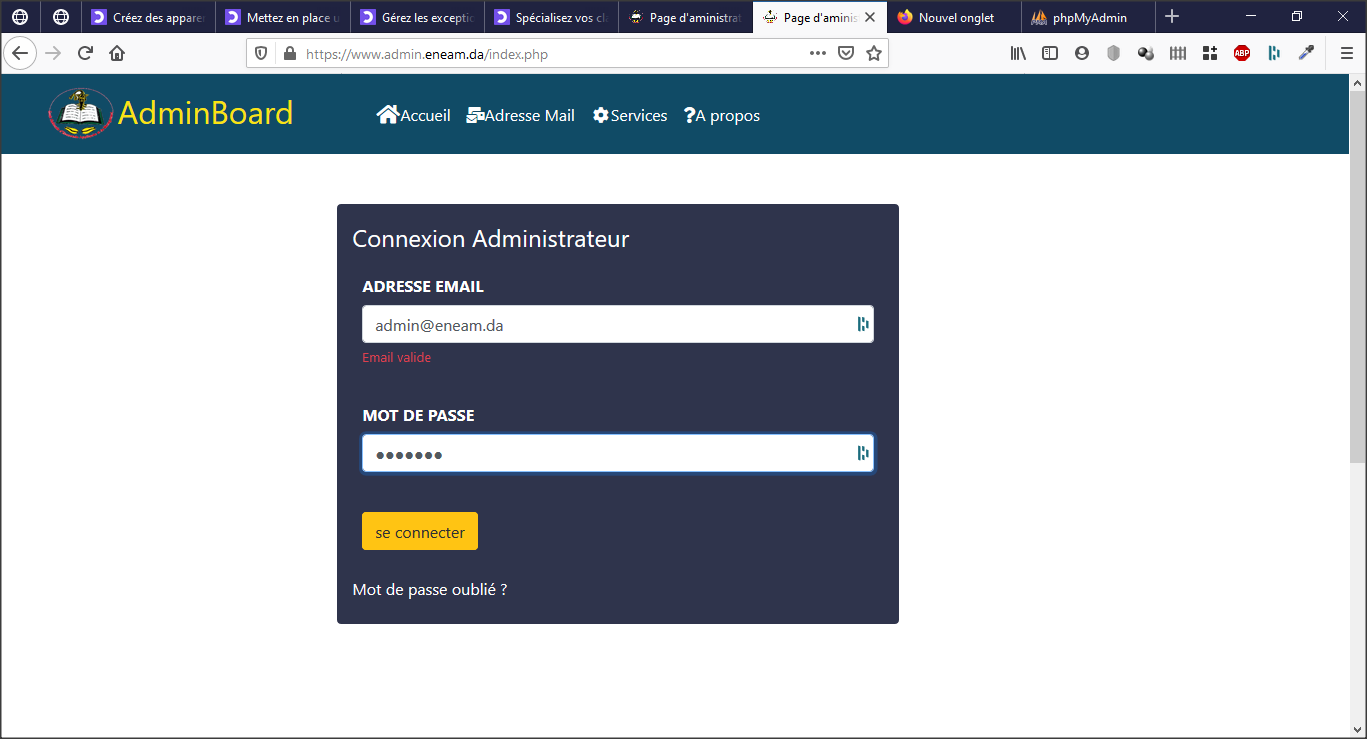
\includegraphics[scale=0.5]{figure/connexion_admin.png}
\caption{Connexion de l'administrateur au site d'administration}
\end{figure}
\item Sur la page d'accueil il renseigne le mail qu'il veut créer. Ici nous allons mettre simplement bake@eneam.da. Puis on renseigne le mot de passe qui doit avoir une forte entropie\footnote{il est obligatoire d'avoir au moins 8 caractères , un caractère spécial, une minuscule et une majuscule}. On suppose ici \emph{Ba21@kesccT}. On confirme le mot de passe.
\item Facultatif: On coche la case Afficher les informations facultatives. Ce qui permet de renseigner le nom et prénom de l'étudiant, son numéro matricule , numéro de téléphone, la date d'expiration du compte.\footnote{Les comptes étant essentiellement pour des étudiants on considère que le compte est valide durant la période d'étude. On utilisera un cron pour désactiver automatiquement les comptes expirés.}
\begin{figure}[H]
\centering
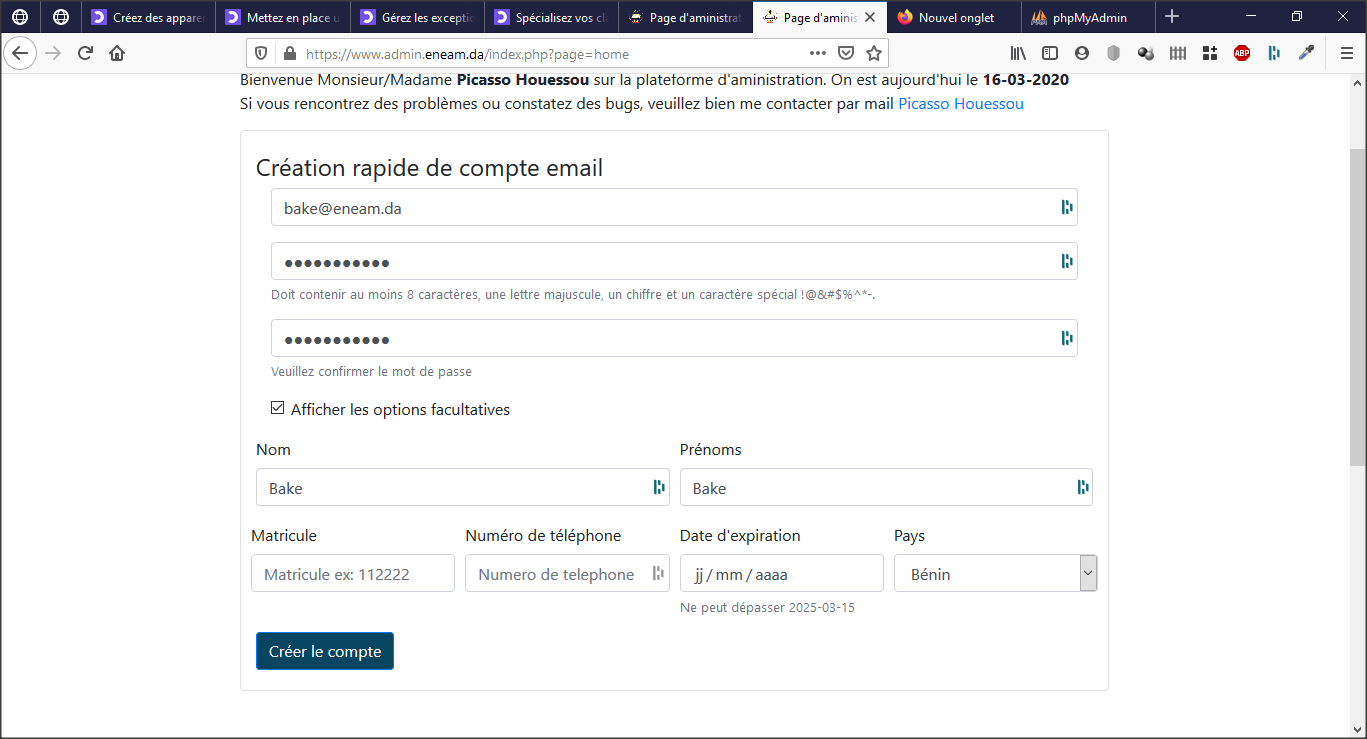
\includegraphics[width=483pt]{figure/creation_compte_bake.png} \\[1cm]
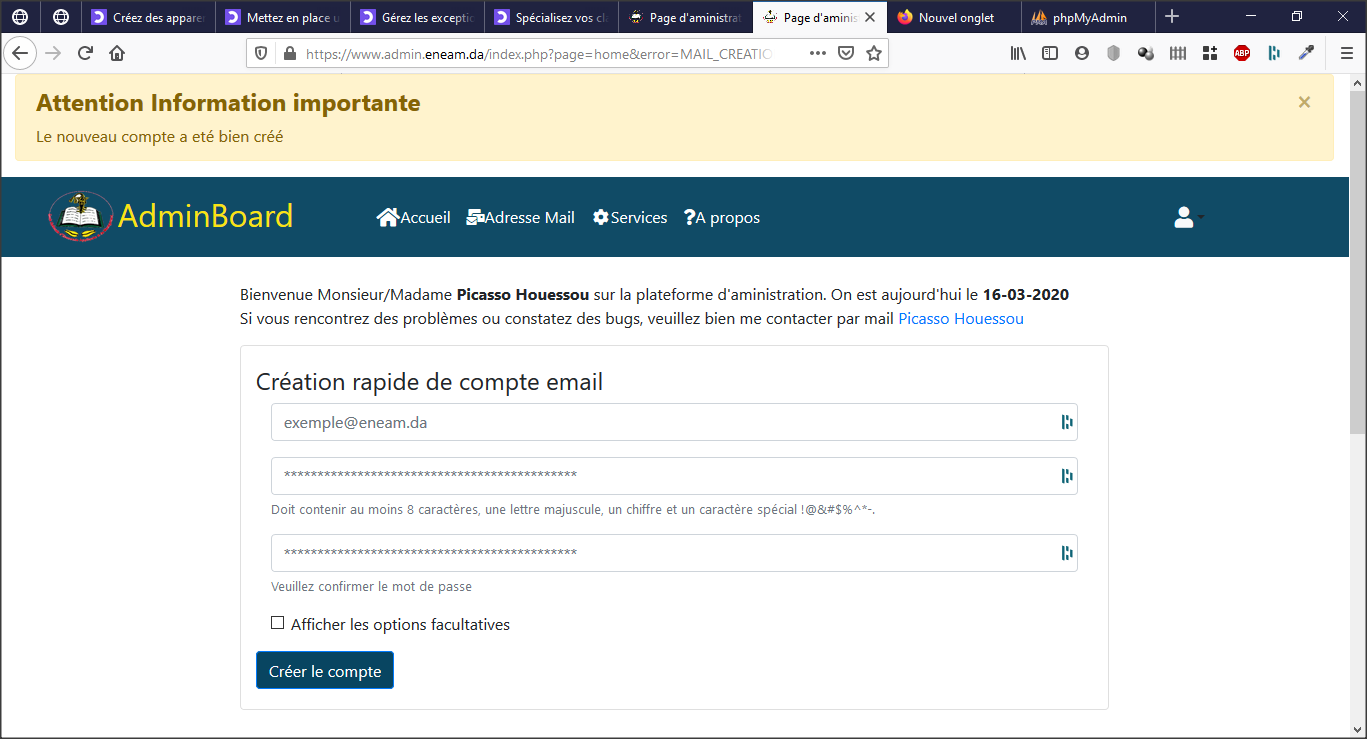
\includegraphics[width=483pt]{figure/retour_compte_cree.png}
\caption{Création du compte bake@eneam.da}
\end{figure} 
\item On appuie sur le bouton \emph{Créer le compte} 
\item Le système renvoie une information pour notifier que le compte à été créé ou s'il a eu une erreur (par exemple si le compte existe déja).
\item Il reprend la même opération pour Toto avec pour adresse mail toto@eneam.da et mot de passe to21@kesccT .
\end{itemize}
\begin{itemize}
\item Baké tape www.eneam.da pour accéder au client webmail. Il saisit ses informations de connexion et se connecte.
\begin{figure}[H]
\centering
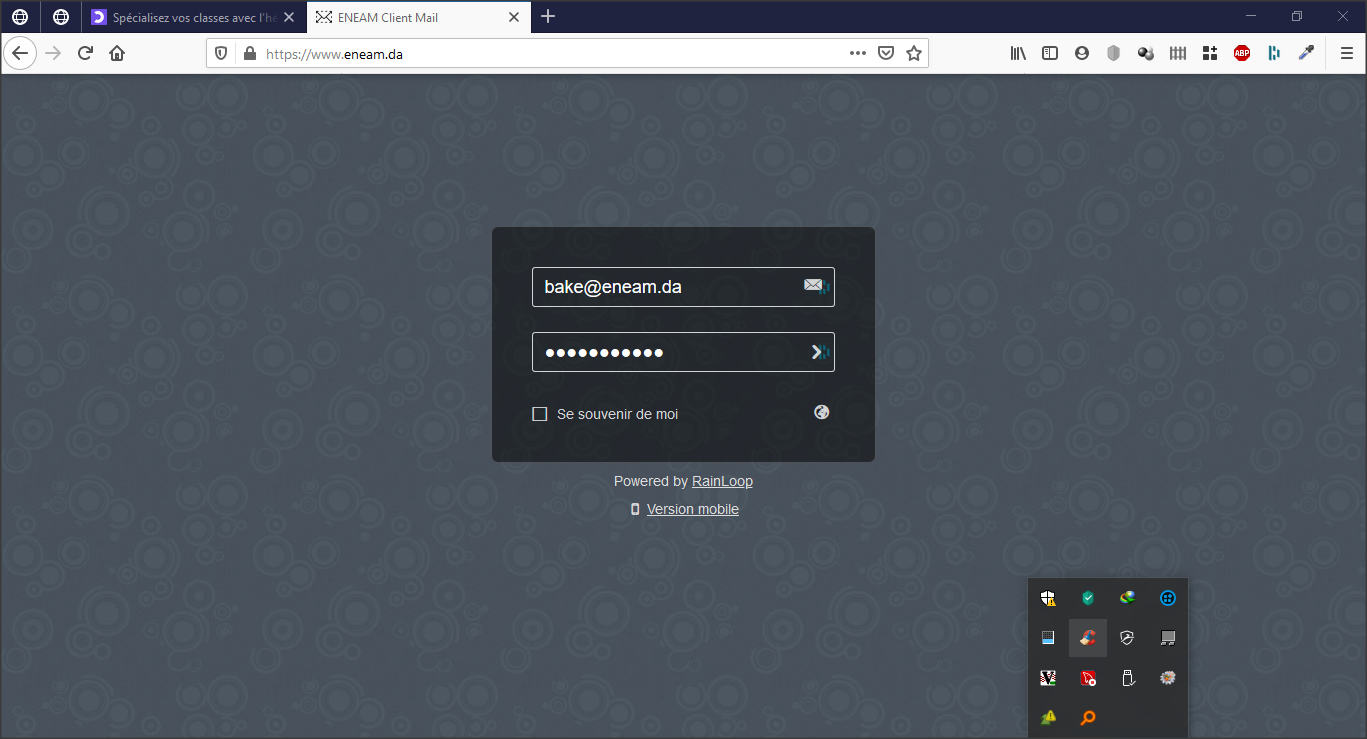
\includegraphics[width=483pt]{figure/connexion_bake_large_screen.png}
\caption{Connexion de Baké au client webmail}
\end{figure} 
\item Il crée un nouveau message à destination de Toto et l'envoie
\begin{figure}[H]
\centering
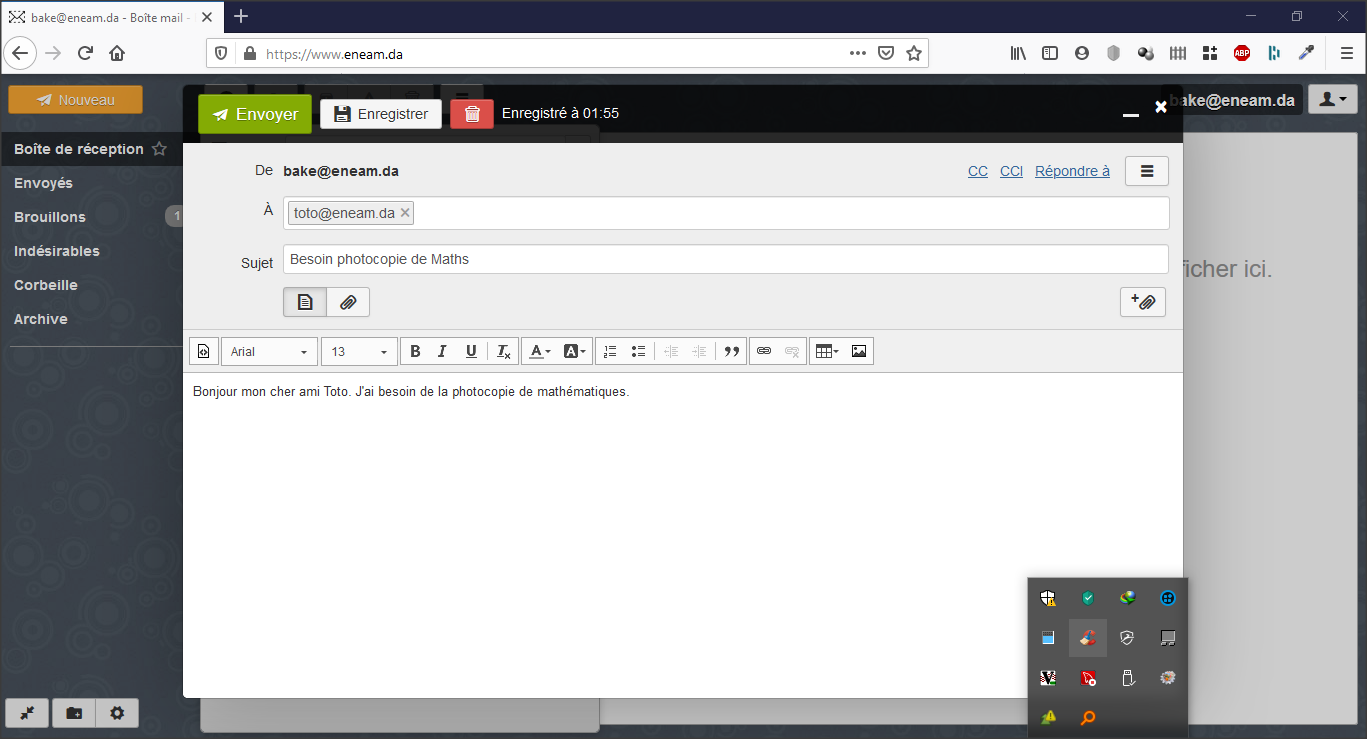
\includegraphics[width=483pt]{figure/bake_send_mail_to_toto1.png}
\caption{Envoi d'un mail de Baké à Toto}
\end{figure}

\item Toto se connecte voit le message et répond.
\begin{figure}[H]
\centering
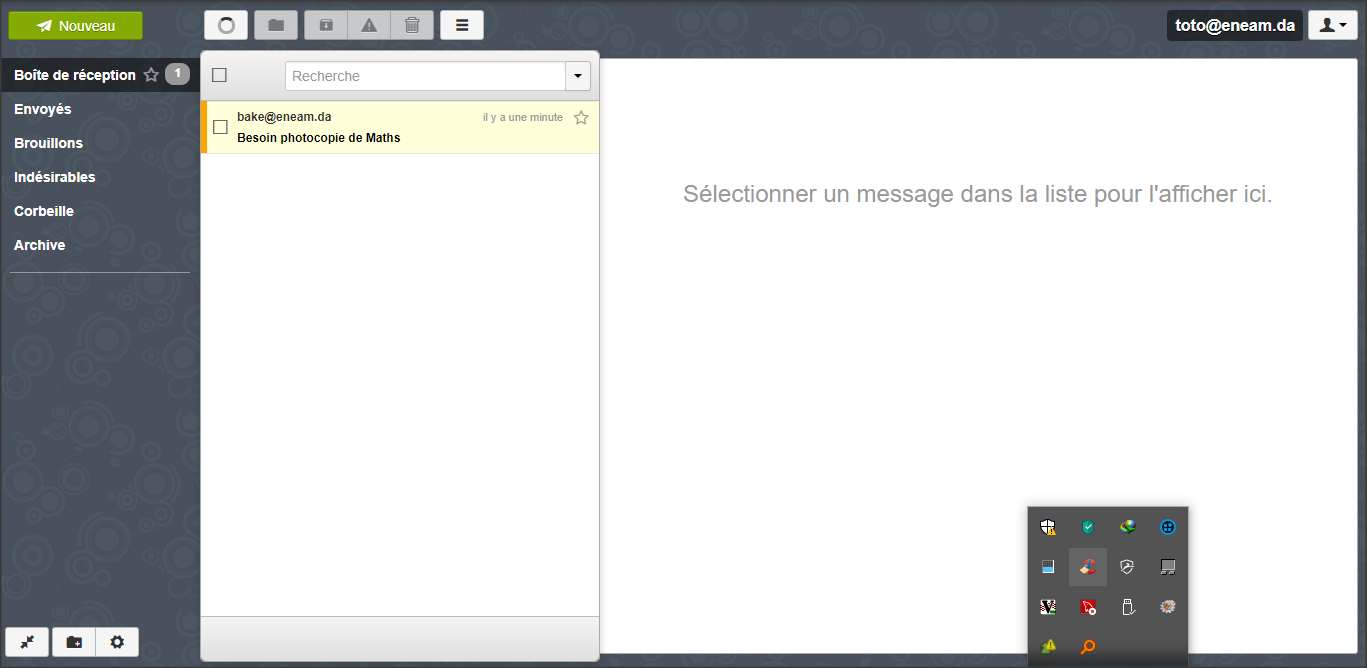
\includegraphics[width=483pt]{figure/toto_see_mail_from_bake1.png} \\[1cm]
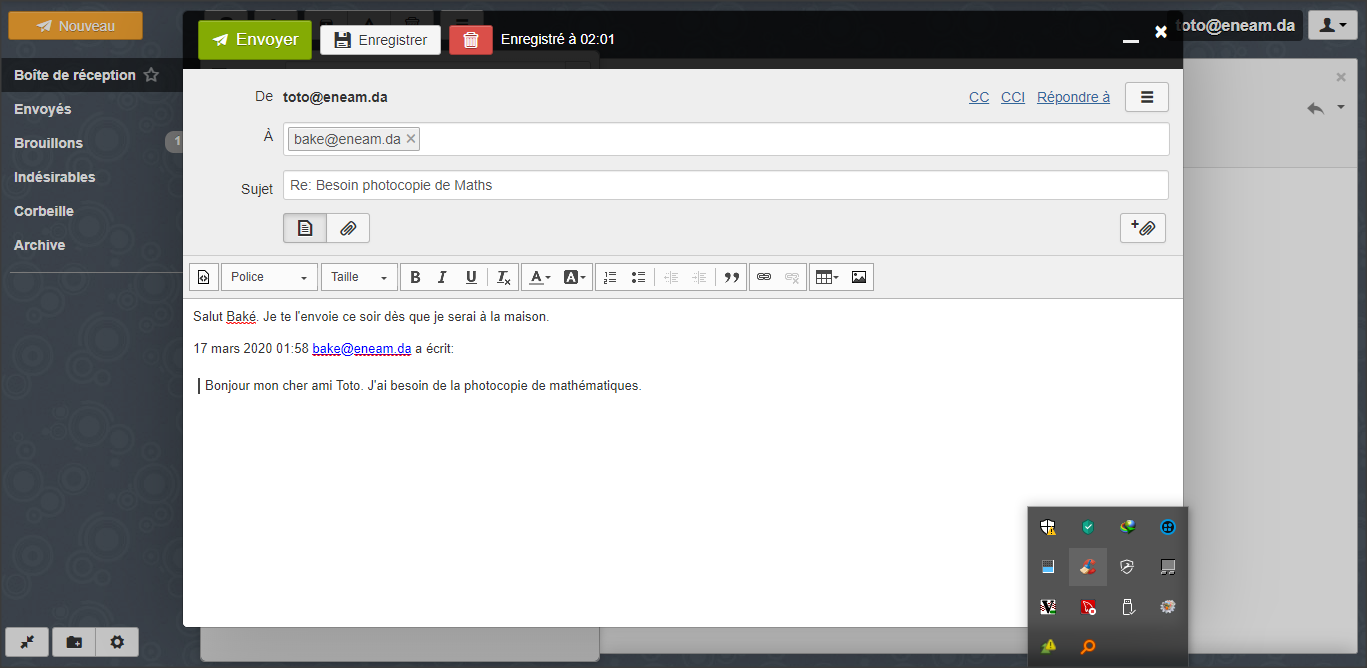
\includegraphics[width=483pt]{figure/toto_reply_to_bake1.png}
\caption{Réponse de Toto au mail de Baké}
\end{figure} 

\item L'administrateur se connecte aussi et envoi un message de convocation à Toto 
\item Toto se connecte voit le message de Baké et répond.
\begin{figure}[H]
\centering
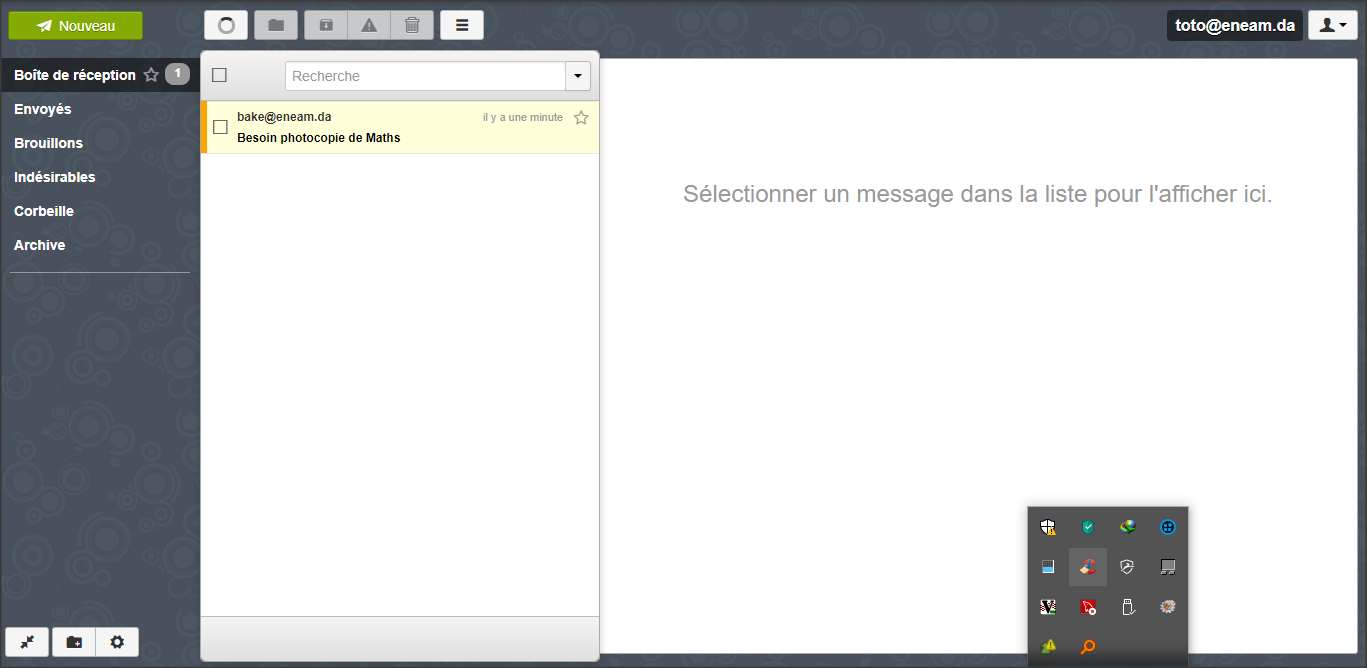
\includegraphics[width=483pt]{figure/toto_see_mail_from_bake1.png} \\[1cm]
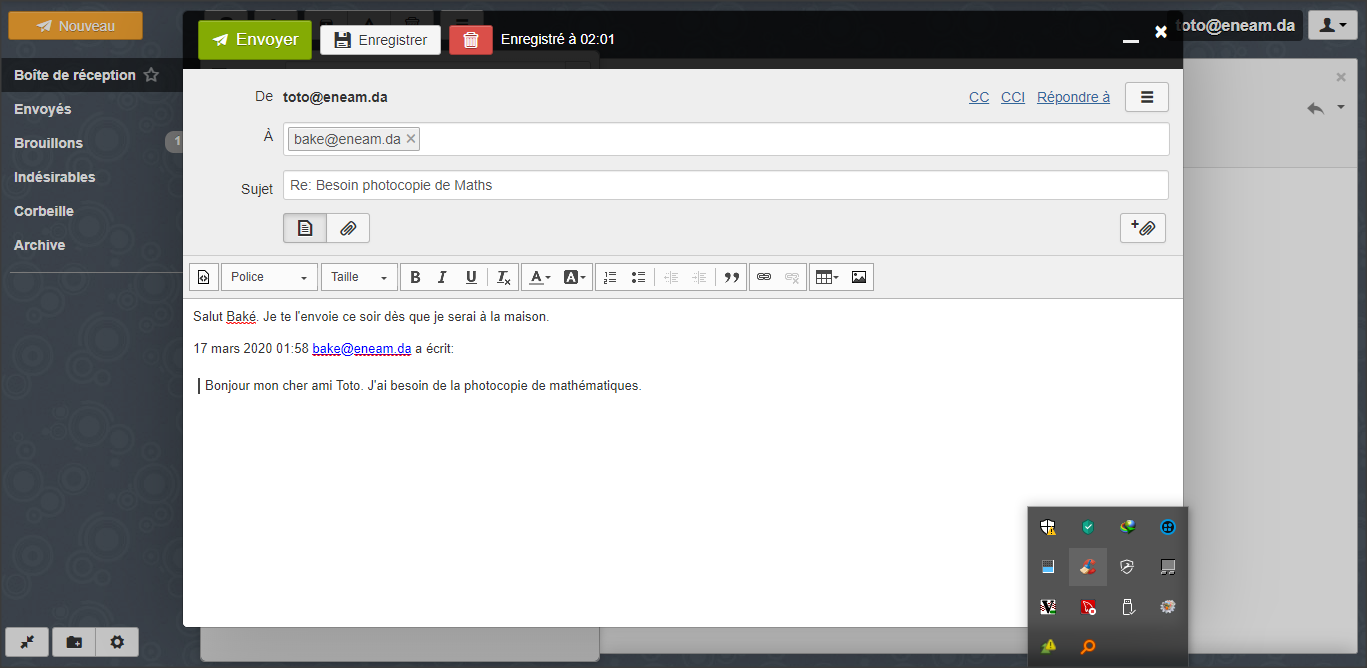
\includegraphics[width=483pt]{figure/toto_reply_to_bake1.png}
\caption{Lecture du mail reçu de Baké par Toto}
\end{figure} 

\item L'administrateur supprime le compte de Béréké : Pour cela il clique sur le menu Adresse mail. Ensuite il recherche le compte de Toto et clique sur le bouton représenté par un bonhomme avec une croix. Une boite de dialogue apparaît et demande de confirmer la suppression. Il clique sur oui supprimer. Des toasts apparaîssent pour notifier si le compte est supprimé. Il a la possibilité de les effacer ou de les enregistrer en un format texte au cas où il voudrait écrire des notes plus tard. 
\begin{figure}[H]
\centering
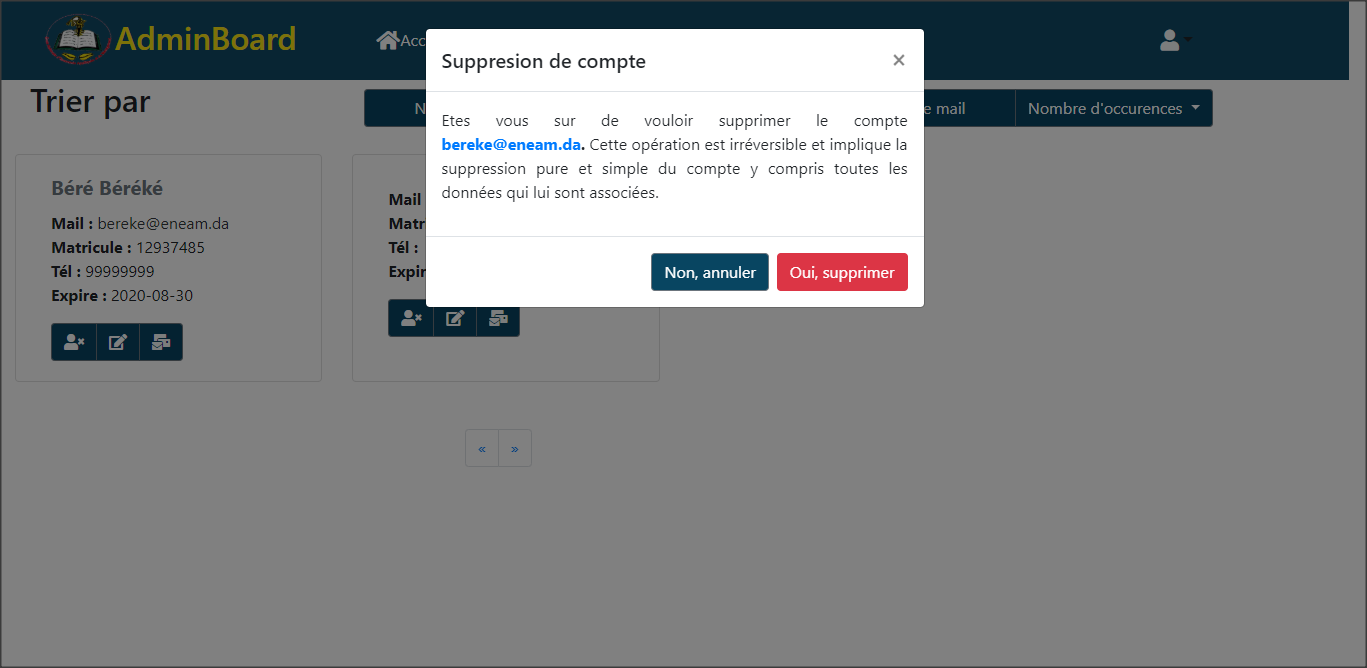
\includegraphics[width=483pt]{figure/admin_delete_bereke_acount1.png} \\[1cm]
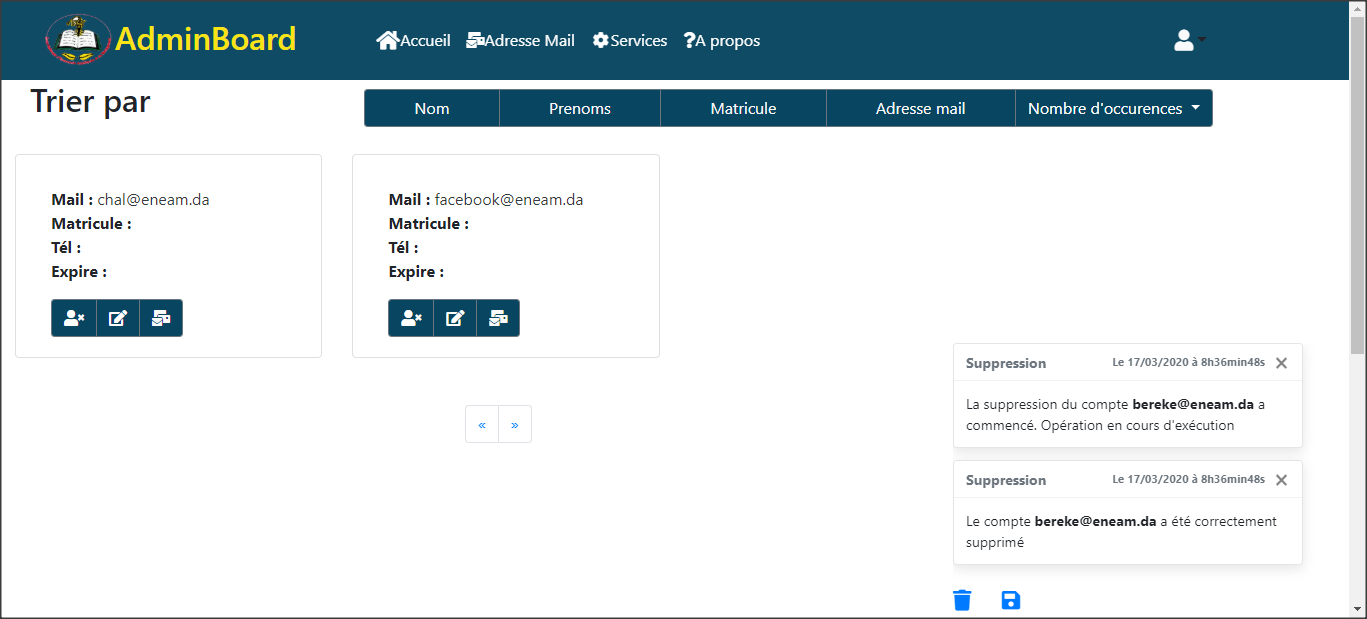
\includegraphics[width=483pt]{figure/admin_delete_bereke_acount2.png}
\caption{Suppression du compte de Béréké}
\end{figure}  

\end{itemize}
\begin{itemize}
\item L'administrateur clique sur le menu Services. Il observe sur cette page 5 services. Le service Apache, Nginx, PHP7.2-FPM, Postfix, Dovecot. Il peut choisir de redémarrer un service en cliquant sur l'icone redémarrer dans le champ correspondant ou redémarrer tous les services à la fois en cliquant sur le bouton redémarrer tous les services. Il peut de même arrêter un service au besoin. Il est impossible d'arrêter les services web (Apache , Nginx, PHP7.2-FPM ). En effet, il contrôle le serveur par l'interface web. S'il arrête donc les services web, il serait impossible de manipuler le serveur depuis le navigateur et il sera bloqué. C'est d'ailleurs la raison pour laquelle l'icône arrêter est désactivé pour ces trois services.
\begin{figure}[H]
\centering
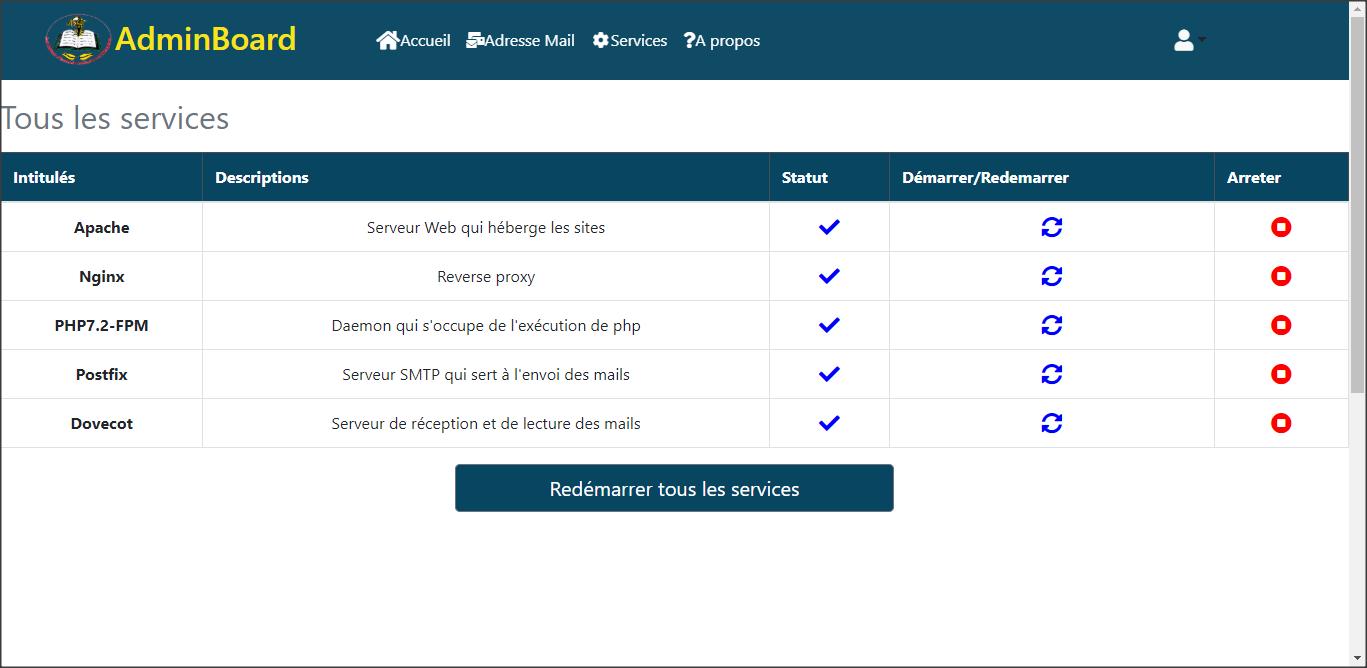
\includegraphics[width=483pt]{figure/admin_verify_state_of_service.png}
\caption{Vérification de l'état des services}
\end{figure}  

\item L'administrateur arrête les services mails( Postfix et dovecot)
\begin{figure}[H]
\centering
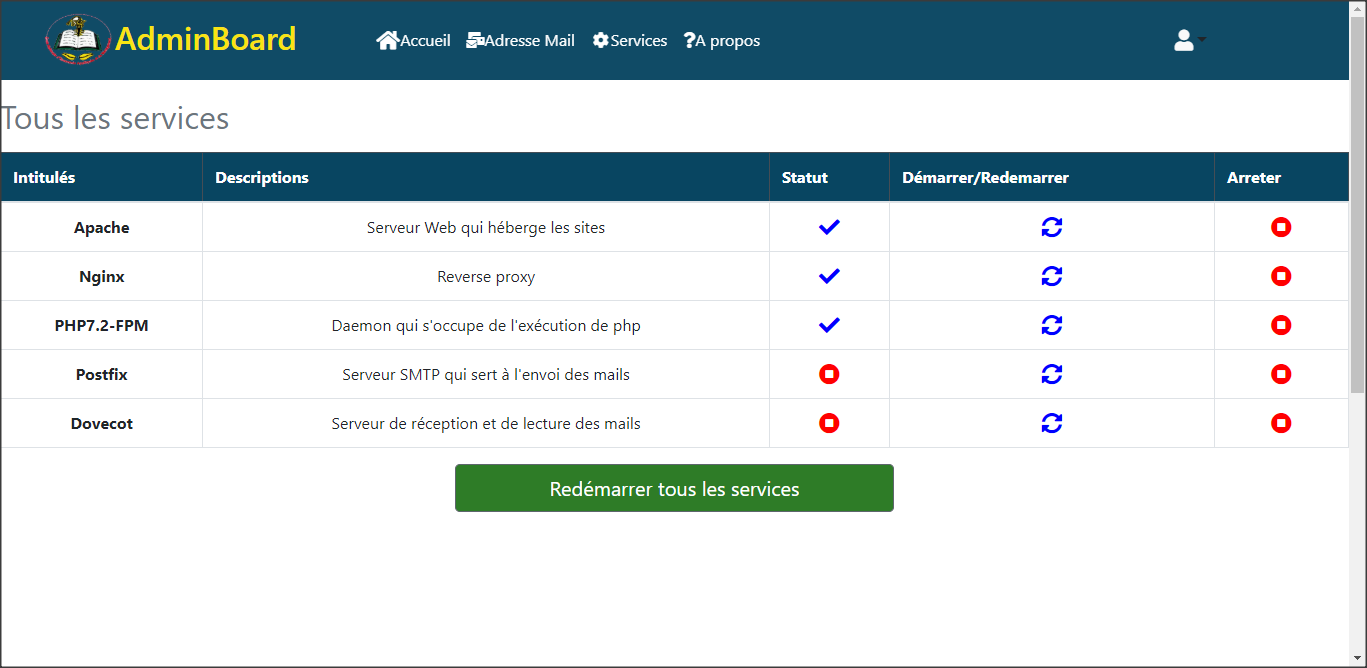
\includegraphics[width=483pt]{figure/admin_stop_service_mail.png}
\caption{Arrêt des services Postfix et Dovecot}
\end{figure}  

\item Il se déconnecte en cliquant sur l'icone située à l'extrême droite de l'écran et en appuyant sur se déconnecter. Pour des raisons de sécurité , il est aussi déconnecté automatiquement après une durée d'inactivité de 15 minutes. 

\end{itemize}
%\inputminted{frame = single, style = vim, autogobble,breaklines, bgcolor=bg, label=Console}{console}{vsftpd}
\chapter*{Conclusion}
Mon stage académique effectué au sein de JScom s'est révélé être une expérience marquante et m'a montré un aperçu des réalités quotidiennes en milieu professionnel.
J'ai mis en place un système d'envoi de mails pour faciliter les échanges au sein de l'ENEAM. Ce qui m'a permis d'explorer le vaste monde de l'administration système sous Linux. J'ai donc pu manipuler et découvrir plusieurs services réseaux. 

\addcontentsline{toc}{chapter}{Conclusion} %Ajout de Introduction dans la table des matieres

%Bibliographie
\nocite{ref1}
\nocite{ref2}
\nocite{ref3}
\nocite{ref4}
\nocite{ref5}
\nocite{ref6}
\nocite{ref7}
\nocite{ref8}
\nocite{ref9}
\nocite{ref10}
\nocite{ref11}
\nocite{ref12}
\nocite{ref13}
\nocite{ref14}
\nocite{ref15}
\nocite{ref16}
\bibliographystyle{plain}
\bibliography{bibliographie} % mon fichier de base de données s'appelle bibliogrphie.bib
\addcontentsline{toc}{chapter}{Bibliographie} %Ajout de Bibliographie dans la table des matieres
%Annexe
\end{document}
